% !TeX program = xelatex
\documentclass[12pt,a4paper]{article}
\usepackage{titlesec}
\titlespacing*{\section}{0pt}{*1}{*1}
\titlespacing*{\subsection}{0pt}{*1}{*1}
\usepackage{xeCJK} % 使用 xeCJK 宏包
\usepackage{fontspec} % 加载字体
\usepackage{indentfirst}
\usepackage{placeins}
\usepackage{pgfplots}
\usepackage{float}
\usepackage{amsmath} % 加载amsmath宏包
\pgfplotsset{compat=newest}

% 设置文档字体
\setCJKmainfont{SimSun} % 设置中文主字体为宋体
\setmainfont{Times New Roman} % 设置英文主字体

% 其他LaTeX包和配置
\usepackage{graphicx} % 用于插入图像
\usepackage{hyperref} % 用于插入超链接
\usepackage{xcolor}
\usepackage{setspace}
\usepackage[margin=0.7in, headheight=5pt, headsep=7pt, footskip=5pt]{geometry}




\title{Notes for Introduction to Economics}
\author{}
\date{}
\begin{document}
\onehalfspacing
\maketitle
\vspace{-3em} % 调整标题后的间距,负值减少空间


% Chapter 1
\section{经济学概述:经济学十大基本原理}

\subsection{人们面临均衡取舍}

\subsection{某些东西的成本是为了得到它所放弃的东西}
\textcolor{red}{机会成本}: 为了得到某种东西所必须放弃的东西。(其他选择中收益最大项的价值)

\subsection{理性人考虑边际量}
\subsubsection{理性人:有目的地尽最大努力实现目标的人。企业希望利润最大化;个人希望幸福最大化。}
\subsubsection{边际量/边际变动(marginal change): 对现有选择的微小调整}
\subsubsection{比较边际收益和边际成本来做决策}
边际收益递减:它描述了在生产过程中,当一个生产要素的投入量增加时,其他要素保持不变,额外产出(边际产出)的增加量将会越来越小。这意味着,每增加一单位的特定资源投入,所获得的额外收益将逐渐减少,前提是其他输入保持不变。
\subsection{人们会对激励做出反应}
激励:引起一个人做出某种行为的某种东西。
\subsection{贸易可以使每个人的状况变得更好}
贸易[自由交换]使人们可以专门生产一种物品或劳务[分工]并用来交换其他物品或劳务,而不必自给自足。
\subsection{市场通常是组织经济活动的一种好方法}
\noindent 计划经济:政府分配经济中的稀缺资源\\
\noindent 市场经济:企业和家庭在物品和服务市场上交易,由他们分散的决策来配置资源。\\

“看不见的手” (the invisible hand)通过价格体系来发挥作用:
\\- 买者与卖者之间的相互作用决定市场价格
\\- 每个价格即反映了物品对于买者的价值,也反映了生产物品的成本
\\- 在许多情况下,价格会自发调整,引导利己的家庭与企业做出使社会经济福利最大化的决策
\\- 通常市场是由竞争来约束利己行为的
\subsection{政府有时可以改善市场结果}
\noindent 政府的一个重要作用:保护产权
\\产权(property rights):个人拥有并控制稀缺资源的权利
\\在某些情况下,市场本身不能有效配置资源,即市场失灵(market failure),此时政府的干预可以改善资源配置。
\subsection{一国的生活水平取决于它生产物品与服务的能力}
生产率(productivity),即每个人或每一单位劳动投入所生产的物品与服务数量
\subsection{当政府发行了过多货币时,物价上升}
通货膨胀(inflation):经济中物价总水平的上升
\subsection{社会面临通货膨胀与失业之间的短期权衡取舍}
\noindent 在短期里,发行货币的效应可能是:
\\- 经济中货币量增加刺激了社会的整体支出水平,从而增加对物品和服务的需求
\\- 引起物价提高;并因此激励企业雇佣更多的工人,生产更多的物品与服务
\\- 企业雇佣更多的工人意味着更少的失业


\subsection{经济学旨在分析社会对稀缺资源的管理,主要研究不同对象如何做\textcolor{red}{决策}
}
Why?资源的稀缺性。
\subsection{微观经济学与宏观经济学}
\noindent 微观经济学(microeconomics):研究家庭和企业如何做出决策,以及它们如何在市场上相互交易\\
宏观经济学(macroeconomics):研究整体经济现象,包括通货膨胀,失业和经济增长
\subsection{经济学三要素:基本概念、原理及模型}
\subsection{实证经济学与规范经济学}
\noindent 实证表述(positive statement):试图描述世界是什么样的观点\\
规范表述(normative statement):试图描述世界应该是什么样的观点
\subsection{循环流量图}
\begin{figure}[H] 
  \centering % 使图片居中显示
  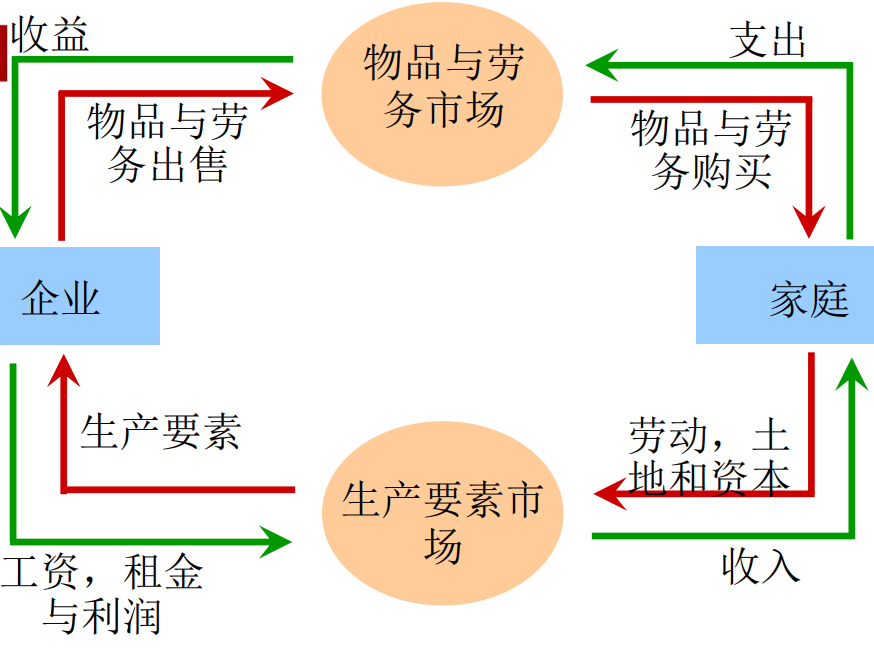
\includegraphics[width=0.4\textwidth]{循环流量图.png} 
  \caption{循环流量图} % 为图片添加标题
\end{figure}


% Chapter 2
\section{贸易与比较优势}


\subsection{生产可能性边界}

\indent\textcolor{red}{生产可能性边界(production possibilities frontier)}:表示在可得到的生产要素与生产技术既定时,一个经济所能生产的两种产品数量的各种组合的图形\\

生产可能性边界上的点代表了有效率的生产水平:在边界上,如不减少一种产品的生产,就不能生产更多的另一产品

生产可能性边界内的点代表了无效率/低效率(inefficient)的结果

\begin{figure}[H] 
  \centering % 使图片居中显示
  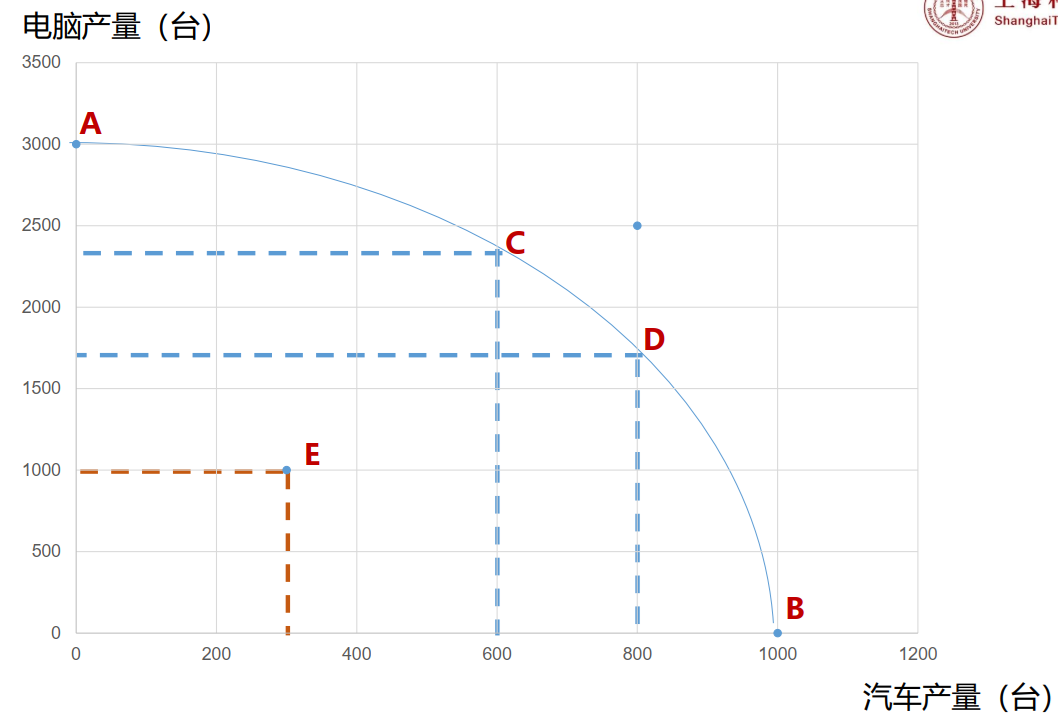
\includegraphics[width=0.8\textwidth]{生产可能性边界.png} % 插入图片,设置图片宽度为文本宽度的 80%
  \caption{生产可能性边界} % 为图片添加标题
  \label{fig:cycle} % 为图片设置标签,用于引用
\end{figure}
\textcolor{red}{机会成本}:机会成本是为了得到某件东西所放弃的东西,例如生产物品A所花的时间可以生产物品B的数量\\

e.g.为了增加400台汽车,我们将减少2400台电脑:平均每台汽车的机会成本是6台电脑\\

生产可能性边界最有可能是向外突出。

当一个经济体的生产技术使得它可以以固定比率转换生产两种商品时,即生产一种商品的增加总是以牺牲另一种商品的固定比率减少为代价,PPF将是一条直线。

\subsection{比较优势与贸易}

\textcolor{red}{绝对优势}:一个生产者用比另一个生产者更少的投入生产某种物品的能力\\

e.g.美国在生产小麦上有绝对优势:美国生产1吨小麦需要10个劳动小时,而在中国需要25个劳动小时\\

\textcolor{red}{比较优势}:一个生产者以低于另一个生产者的机会成本生产一种物品的能力\\

e.g.生产1台电脑的机会成本:

• 美国是10吨小麦,因为美国生产1台电脑需要100个劳动小时,而100个劳动小时可以生产10吨小麦

• 中国是5吨小麦,因为中国生产1台电脑需要125个小时,而125个小时能够生产5吨小麦

• 因此,中国在生产电脑上有比较优势\\

每个国家应该专门生产其比较优势较大的产品。当每个国家专门生产它具有比较优势的物品时,所有国家的总产量会更高,世界的“经济蛋糕”也会更大,通过贸易也可以使每个人的状况变得更好

\begin{figure}[H] 
  \centering % 使图片居中显示
  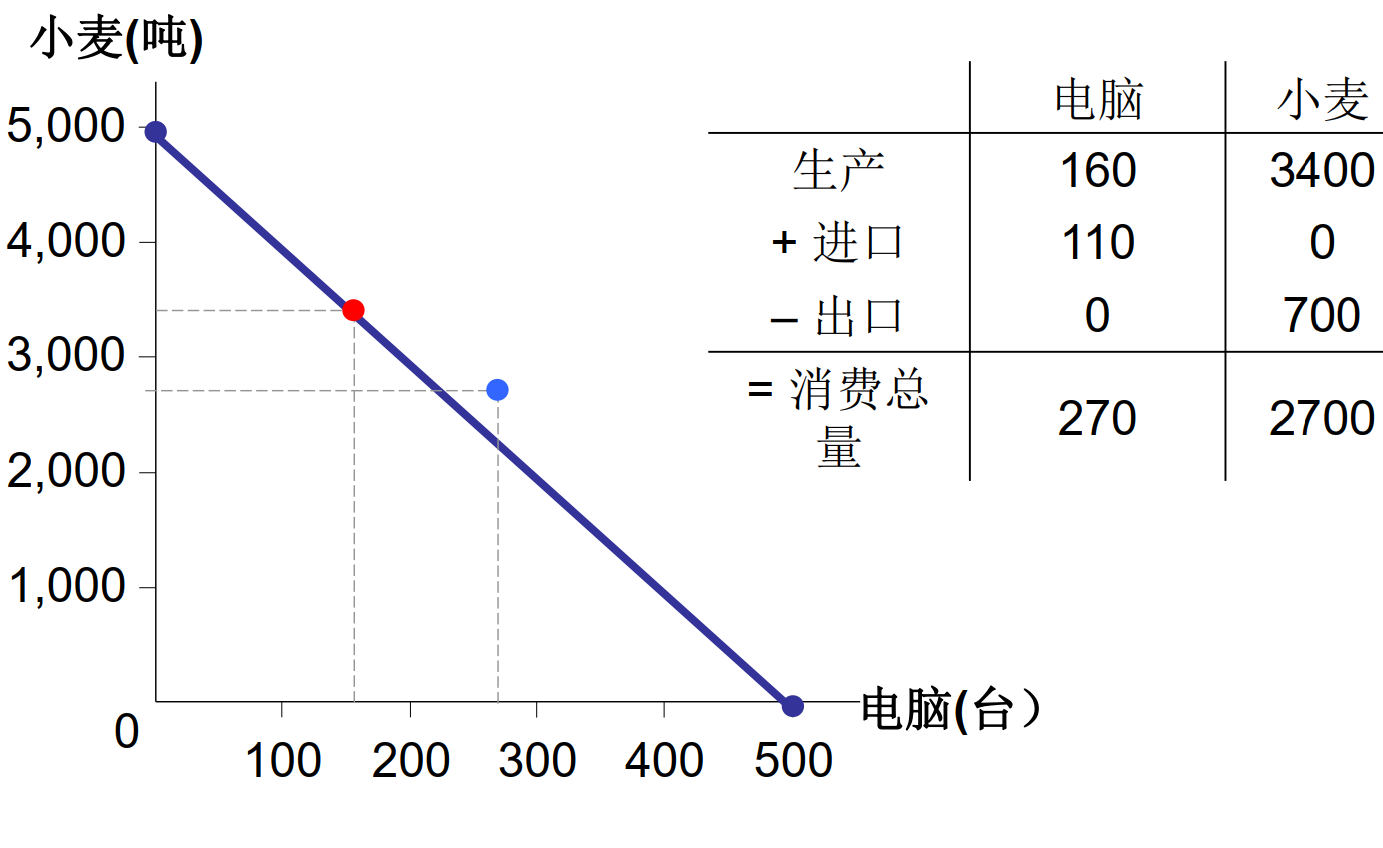
\includegraphics[width=0.4\textwidth]{贸易的好处.png} % 插入图片,设置图片宽度为文本宽度的 80%
  \caption{贸易的好处} % 为图片添加标题
\end{figure}

% Chpter 3 供给与需求

\section{供给与需求}
% 3.1
\subsection{市场与竞争}
市场是由某种物品或服务的买者与卖者组成的一个群体;买者作为一个群体决定了需求,卖者作为一个群体决定了供给。\\

\textcolor{red}{完全竞争市场的特点}:\\
1. 可供销售的物品是完全相同的\\
2. 买者与卖者人数众多, 以至于没有任何一个买者或卖者可以影响市场价格,也就是说,每个人都是“价格接受者” (price taker)\\
3. 资源自由流动,市场信息畅通\\

%3.2需求与供给
\subsection{需求与供给}
%3.2.1需求
\subsubsection{需求(Demand)}
需求量(quantity demanded): 买者愿意并且能够购买的一种物品的数量\\ 

需求定理(Law of Demand):在其他条件不变时,一种物品的价格上升,对该物品的需求量将减少 [价格可以看成机会成本]\\

市场需求是所有个人对某种特定物品或服务的需求的总和\\
%3.2.2需求曲线
\subsubsection{需求曲线 (Demand Curve)}
需求表对应了需求曲线;根据习惯,我们让纵轴代表价格(P),横轴代表数量(Q)\\

\begin{figure}[H] 
  \centering % 使图片居中显示
  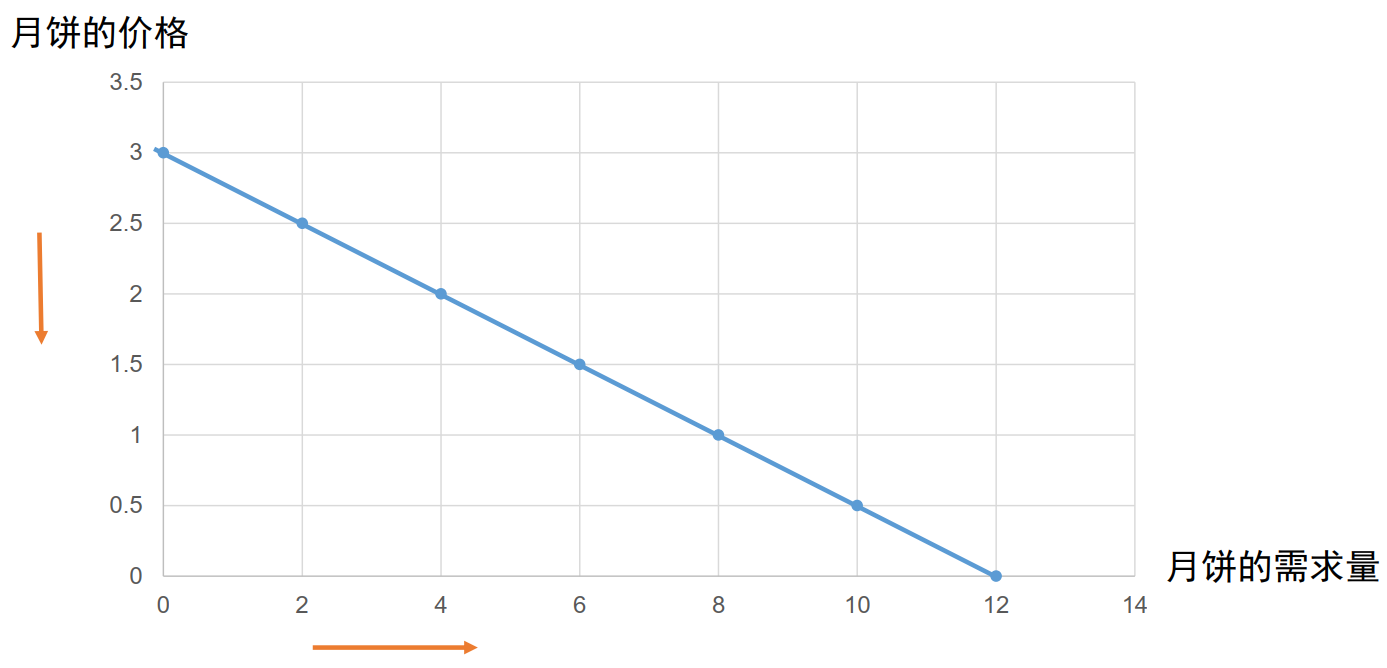
\includegraphics[width=0.6\textwidth]{需求曲线.png} % 插入图片,设置图片宽度为文本宽度的%
  \caption{需求曲线} % 为图片添加标题
\end{figure}

需求曲线的移动:\\

\begin{figure}[H] 
  \centering % 使图片居中显示
  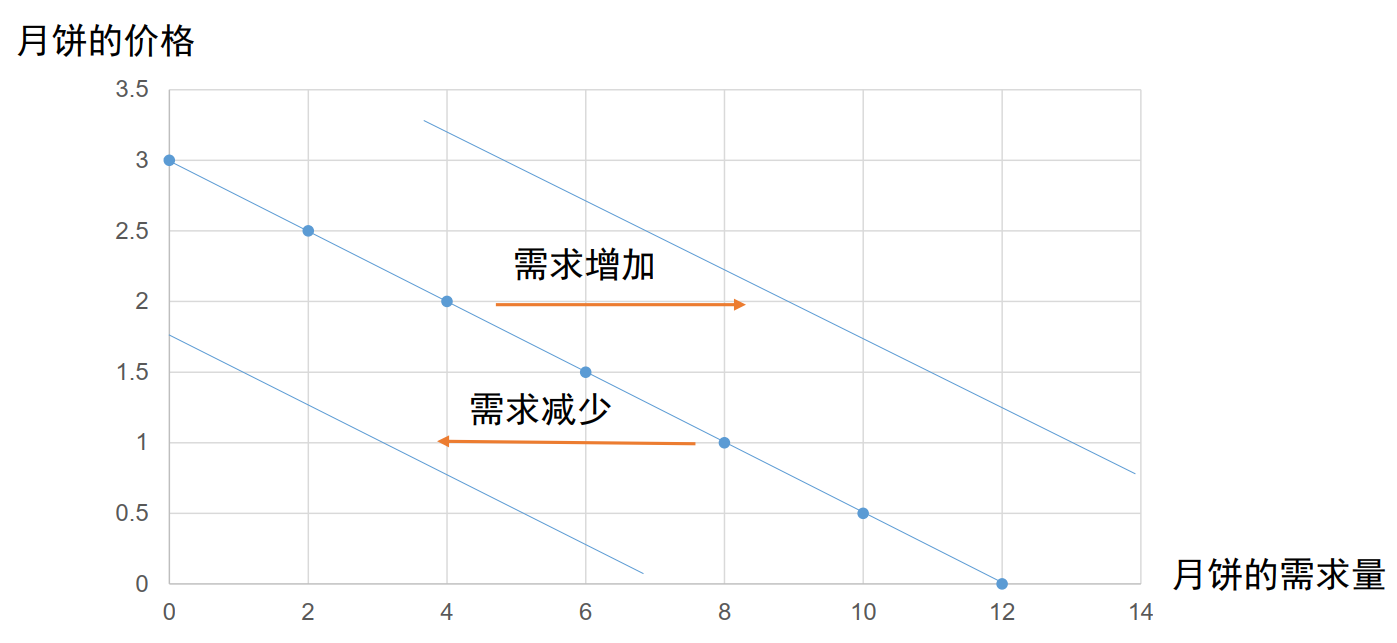
\includegraphics[width=0.6\textwidth]{需求曲线的移动.png} % 插入图片,设置图片宽度为文本宽度的%
  \caption{需求曲线的移动} % 为图片添加标题
\end{figure}

引起需求曲线移动的因素:\\

1. 收入\\
收入降低意味着你的总购买力减少,因此你不得不在某些物品上,也是大多数物品上减少一些支出\\
正常物品(normal good):在其他条件相同时,收入减少引起需求量减少的物品\\
低档物品(inferior good):在其他条件相同时,收入减少引起需求量增加的物品\\

2. 相关物品的价格\\
当一种物品价格上升/下降引起对另一种物品需求量增加/减少,这两种物品被称为替代品(substitute)\\
当一种物品价格下降/上升引起对另一种物品需求量增加/减少,这两种物品被称为互补品(complements)\\

3. 偏好\\
经济学实在解释不了… e.g. 阿特金斯饮食法在90年代开始流行,这引起对鸡蛋的需求增加,使鸡蛋的需求曲线向右移动\\

4. 预期\\
e.g. 预期下个月挣工资→现在花更多钱淘宝;预期双11东西会打折→十月份就先忍一忍\\

5. 买者的数量\\
买者数量的增减会影响市场需求的大小\\

\textcolor{red}{价格的变化不会引起需求曲线的变化。}价格变动只表现为沿着需求曲线的移动其他所有因素的影响表现为整条需求曲线的移动。\\


%3.2.3供给
\subsubsection{供给 (Supply)}
供给量(quantity supplied):卖者愿意并且能够出售的该种物品的数量\\

供给定理:在其他条件不变时,一种物品价格上升,该物品供给量将增加

%3.2.4供给曲线
\subsubsection{供给曲线 (Supply Curve)}
供给表对应了供给曲线;根据习惯,我们让纵轴代表价格(P),横轴代表数量(Q)

\begin{figure}[H] 
  \centering % 使图片居中显示
  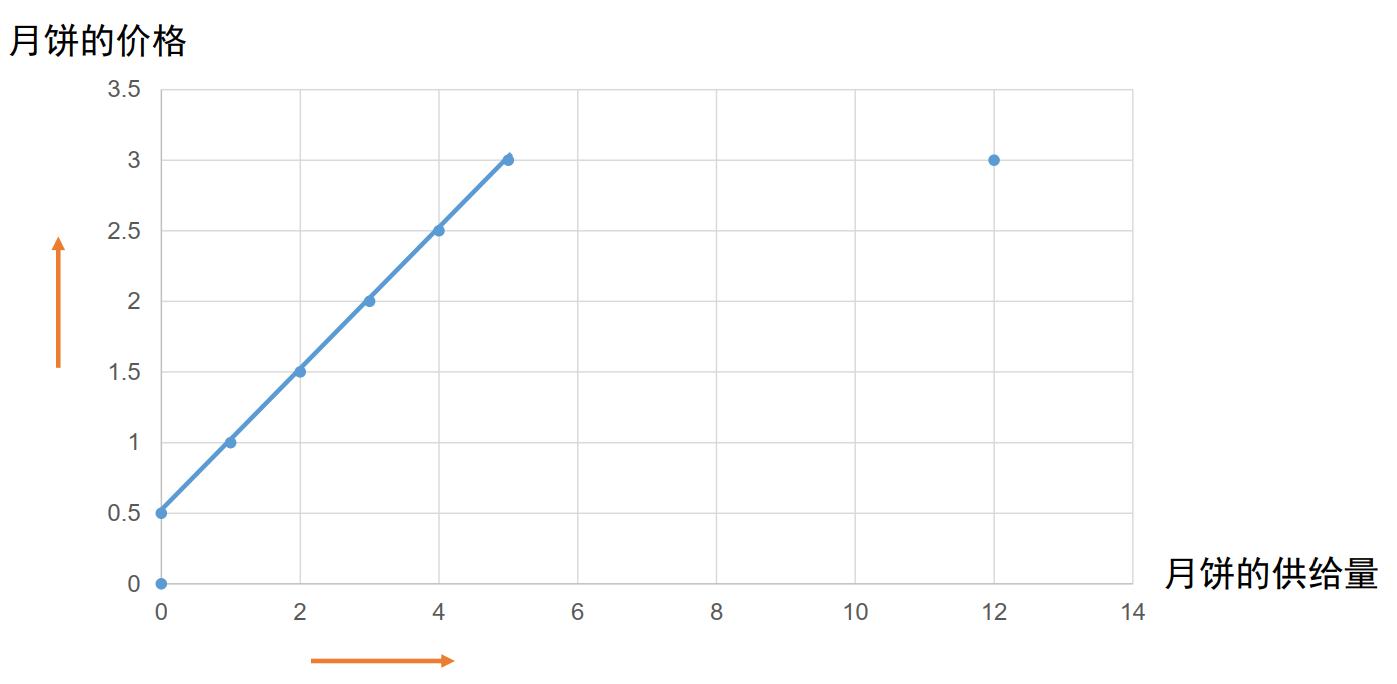
\includegraphics[width=0.6\textwidth]{供给曲线.png} % 插入图片,设置图片宽度为文本宽度的%
  \caption{供给曲线} % 为图片添加标题
\end{figure}

供给曲线的移动:\\

\begin{figure}[H] 
  \centering % 使图片居中显示
  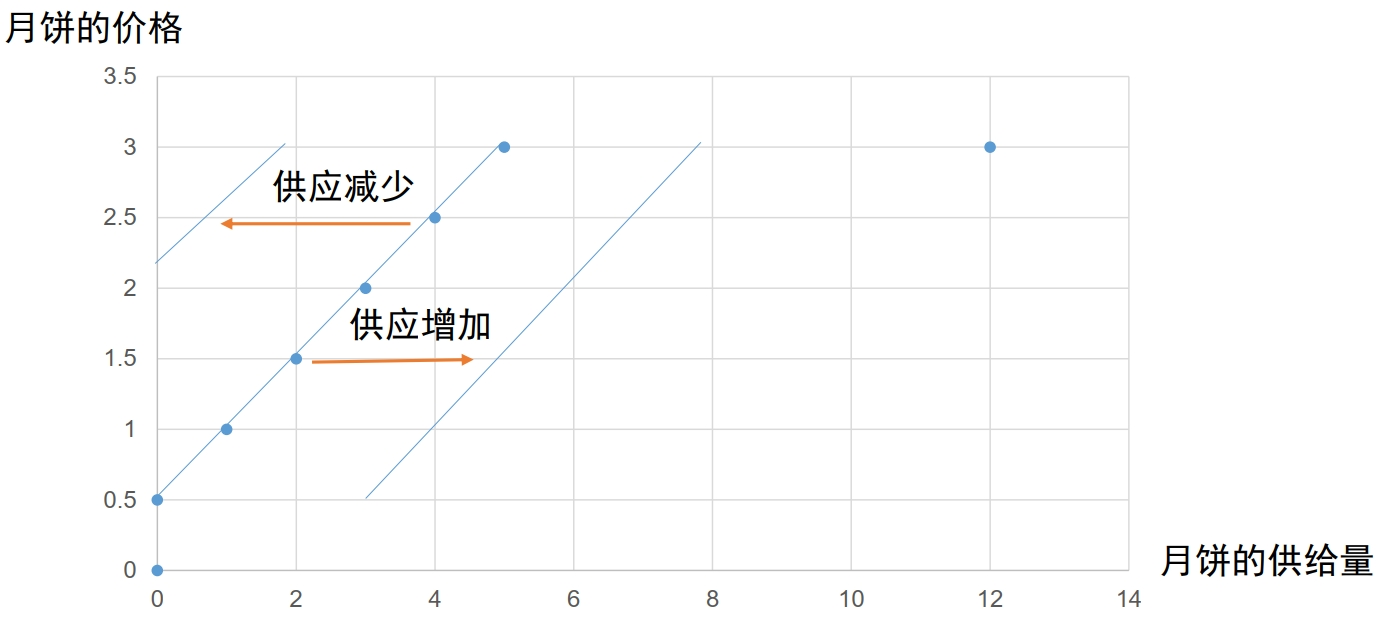
\includegraphics[width=0.6\textwidth]{供给曲线的移动.png} % 插入图片,设置图片宽度为文本宽度的%
  \caption{供给曲线的移动} % 为图片添加标题
\end{figure}

引起供应曲线移动的因素:\\

1. 投入品价格\\
投入品价格上升→相同价格下供应量减少→供应曲线左移\\
投入品价格下降→相同价格下供应量增加→供应曲线右移\\

2. 技术: e.g. 技术进步降低企业的生产成本→供给增加\\

3. 预期: e.g. 如果预期未来冰激凌的价格会上升,企业就会把现在生产的一些冰激凌储存起来,而减少当前的市场供给\\

4. 卖者的数量:卖者数量的增减会影响市场供给的大小\\

\textcolor{red}{价格的变化不会引起供应曲线的变化。}\\

%3.2.5供给与需求的均衡
\subsubsection{供给与需求的均衡}
市场的供给曲线与需求曲线相较于一点,这一点被称为市场的均衡\\

\textcolor{red}{均衡(equilibrium)}:市场价格达到使供给量与需求量相等时的状态\\

\noindent• 市场均衡时的价格称为均衡价格(equilibrium price),均衡价格下的供给量与需求量称为均衡数量(equilibrium quantity)\\
• 均衡价格有时也被称为市场出清价格(clearing price):在这一价格下,买者们买到了他们想买的所有东西,卖者们卖出了他们想卖的所有东西。
\begin{figure}[H] 
  \centering % 使图片居中显示
  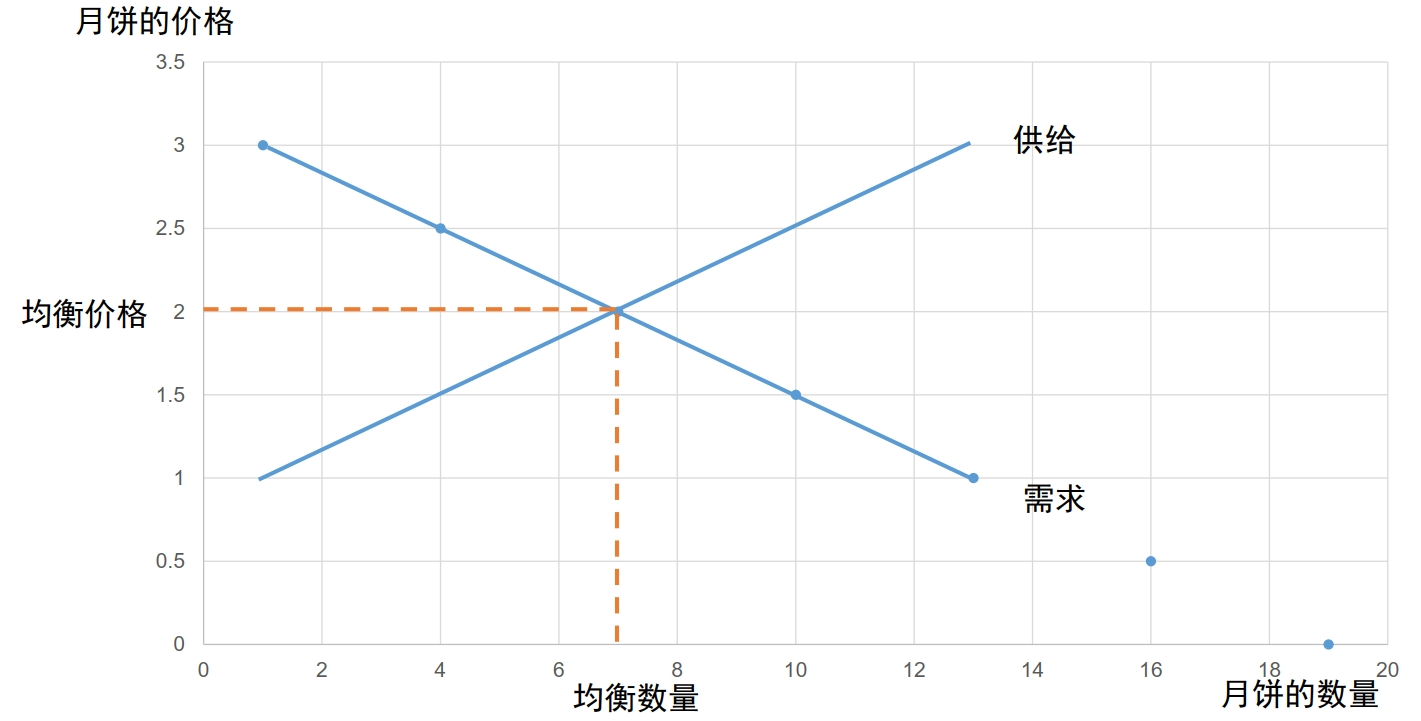
\includegraphics[width=0.6\textwidth]{均衡.png} % 插入图片,设置图片宽度为文本宽度的%
  \caption{均衡} % 为图片添加标题
  \label{fig:equilibrium} % 为图片设置标签,用于引用
\end{figure}

市场会自然而然地向均衡靠拢:\\

\noindent1. 面临过剩,卖者会通过降低价格来增加销量。这会使供给量减少,而需求量增加,价格会持续下降直到市场达到均衡。\\
2. 面临短缺, 卖者会提高价格来增加收入,买者也会愿意付出更高的价格。这会使供给量增加,而需求量减少,价格会持续上升直到市场达到均衡。\\

%3.2.6分析均衡的变动
\subsubsection{分析均衡变动的步骤}
\noindent1. 确定该事件是使供给曲线移动还是使需求曲线移动(还是使两者都移动)\\
2. 确定曲线移动的方向\\
3. 用供求图说明这种移动如何改变均衡价格和均衡数量\\

e.g.事件分析: 汽油价格上升与新技术降低生产成本\\

\begin{figure}[H] 
  \centering % 使图片居中显示
  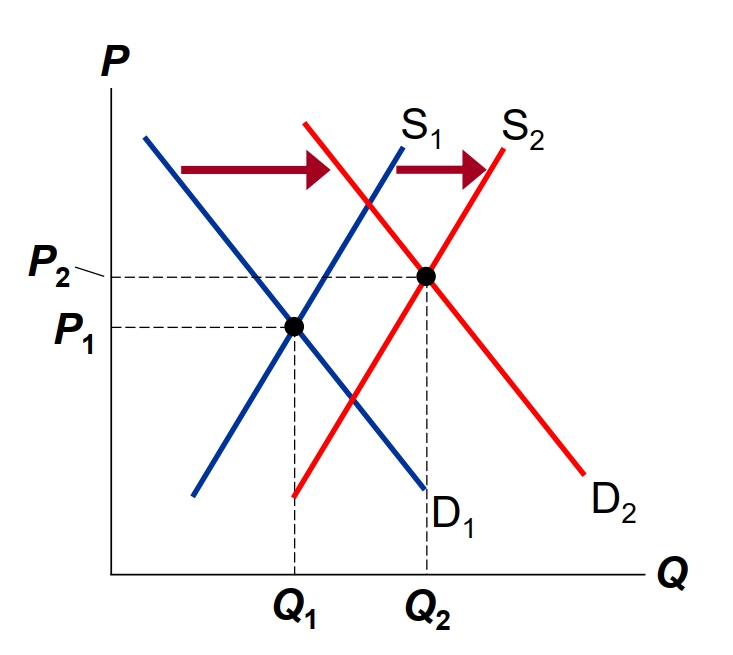
\includegraphics[width=0.4\textwidth]{均衡分析.png} % 插入图片,设置图片宽度为文本宽度的%
  \caption{均衡分析} % 为图片添加标题
\end{figure}

\noindent 第1步:两条曲线都移动\\
第2步:两条曲线都向右移动\\
第3步: 均衡数量增加,但均衡价格的变化不确定。如果需求相对于供给增加的更多,那价格上升;反之亦然。\\

%3.3弹性
\subsection{弹性}

%3.3.1需求价格弹性
\subsubsection{需求价格弹性}
\textcolor{red}{需求价格弹性(price elasticity of demand)}衡量需求量对价格变动的反应程度\\

$$E_d = \left| \frac{\Delta Q / Q}{\Delta P / P} \right| = \left| \frac{\Delta Q}{\Delta P} \cdot \frac{P}{Q} \right|$$

简单的说,它衡量买者需求的价格敏感程度:如果一种物品的需求量对价格变动的反应很大,则这种物品的需求是富有弹性的;反之则是缺乏弹性的\\

\textcolor{red}{中点法求弹性}:\\

计算某一段需求曲线或供给曲线上两点之间的平均弹性\\

$$E_d = \frac{\frac{Q_2 - Q_1}{\frac{Q_2 + Q_1}{2}}}{\frac{P_2 - P_1}{\frac{P_2 + P_1}{2}}}$$

\textcolor{red}{点价格弹性}:\\

在需求曲线上某一特定点处,需求量对价格的敏感程度。它测量的是在这一点上,价格变动一个非常小的单位时,需求量将如何相应地变化\\

$$E_d = \frac{dQ}{dP} \times \frac{P}{Q}$$

需求价格弹性的决定因素:\\
1. 相近替代品的可获得性:有相近替代品的物品的需求往往较富有弹性,因为消费者从这种物品转向其他物品较为容易\\
2. 必需品与奢侈品:必需品的需求往往缺乏弹性,而奢侈品的需求往往富有弹性\\
3. 市场的定义:狭窄定义的市场的需求弹性往往大于宽泛定义的市场的需求弹性,因为狭窄定义的市场上的物品更容易找到替代品\\
4. 时间范围:物品的需求往往在长期更具有弹性 e.g.汽油价格上涨,短期内汽油的需求量只是略有下降。但长期的话, 人们可以购买省油的小排量汽车或搬到上班地方附近居住 ,汽油需求量会更大幅度的减少\\

当弹性大于1,即需求量的变动的比例大于价格变动的比例,需求是富有弹性的;当弹性小于1,即需求量的变动的比例小于价格变动的比例,需
求是缺乏弹性的;当弹性等于1时,即需求量与价格等比例变动时,我们说需求具有单位弹性\\

\begin{figure}[H] 
  \centering % 使图片居中显示
  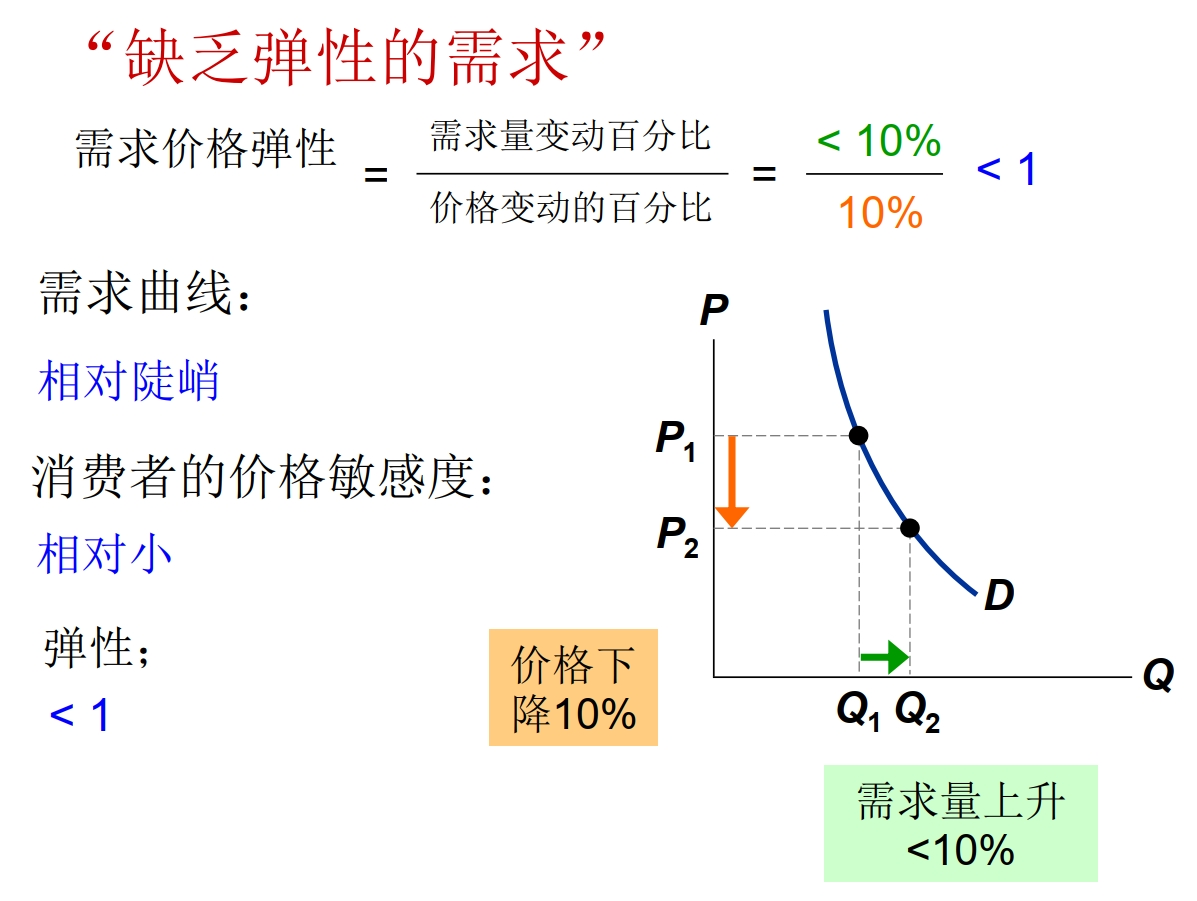
\includegraphics[width=0.6\textwidth]{缺乏弹性的需求.png} % 插入图片,设置图片宽度为文本宽度的%
  \caption{缺乏弹性的需求} % 为图片添加标题
\end{figure}
\begin{figure}[H] 
  \centering % 使图片居中显示
  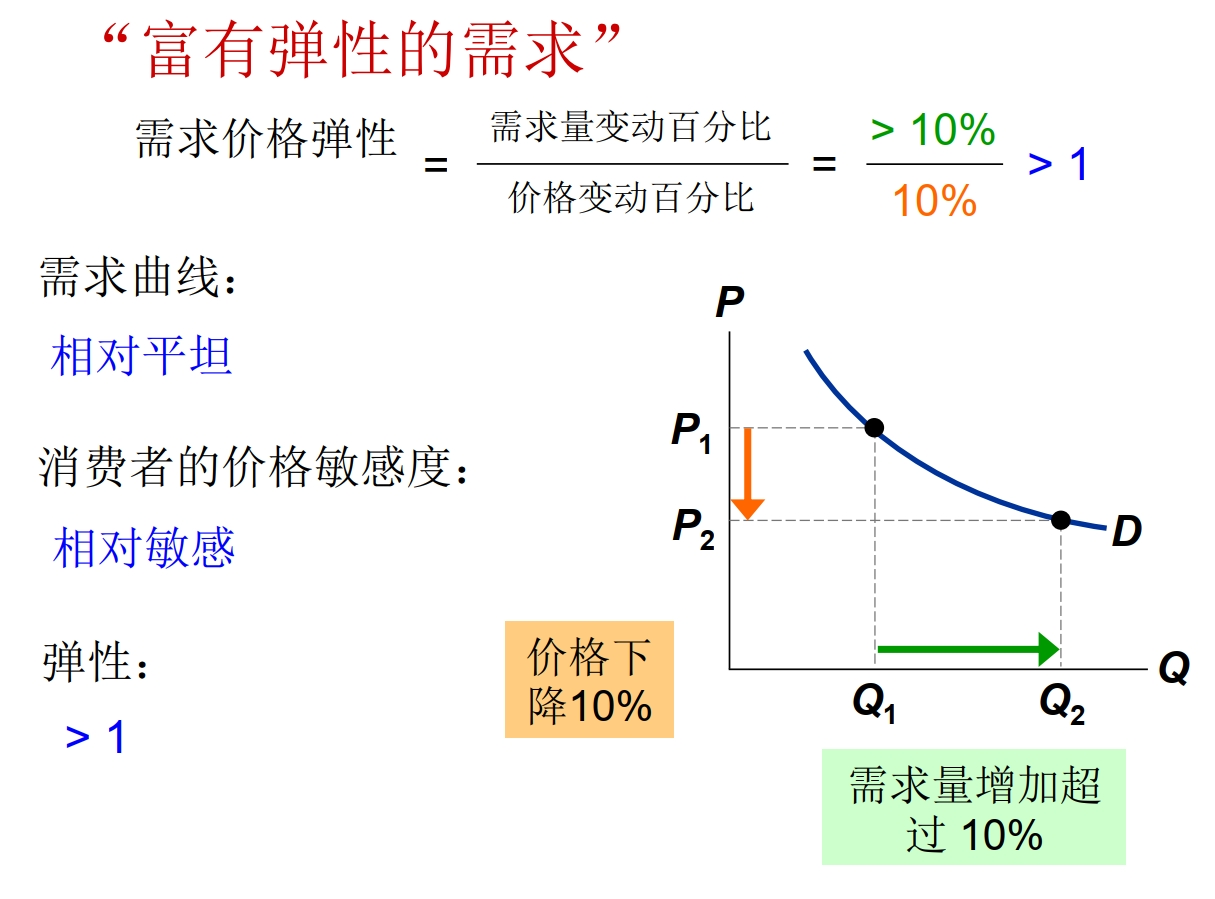
\includegraphics[width=0.6\textwidth]{富有弹性的需求.png} % 插入图片,设置图片宽度为文本宽度的%
  \caption{富有弹性的需求} % 为图片添加标题
\end{figure}

线性需求曲线的弹性\\

线性需求曲线通常表示为 $Q = a - bP$,其中 $Q$ 是需求量,$P$ 是价格,$a$ 和 $b$ 是常数。这样的需求曲线在整个区间上斜率是恒定的,但其价格弹性并不是恒定的。对于线性需求曲线,其点价格弹性的公式可以表示为:

\[ E_d = \frac{dQ}{dP} \times \frac{P}{Q} = -b \times \frac{P}{Q} \]

这里,$-b$ 是需求曲线的斜率,而 $\frac{P}{Q}$ 是给定点上的价格与需求量的比率。

弹性随着价格和需求量的变化而变化:
\begin{itemize}
    \item 当价格很高,需求量很低时(即在需求曲线的左上方),$\frac{P}{Q}$ 的值较大,这使得弹性的绝对值大于 1,表明需求在这一区域是弹性的。
    \item 当价格降低,需求量增加时(即在需求曲线的右下方),$\frac{P}{Q}$ 的值减小,弹性的绝对值也随之减小,需求变得更加无弹性。
    \item 在需求曲线的中点,弹性的绝对值正好等于 1,这个点称为单位弹性点。
\end{itemize}

因此,虽然线性需求曲线的斜率是固定的,其价格弹性却在不同的价格水平上有所不同,从完全弹性(绝对弹性无穷大)到完全无弹性(弹性为零),再到单位弹性,反映了不同价格水平下消费者对价格变化的敏感程度的变化。

\begin{figure}[H] 
  \centering % 使图片居中显示
  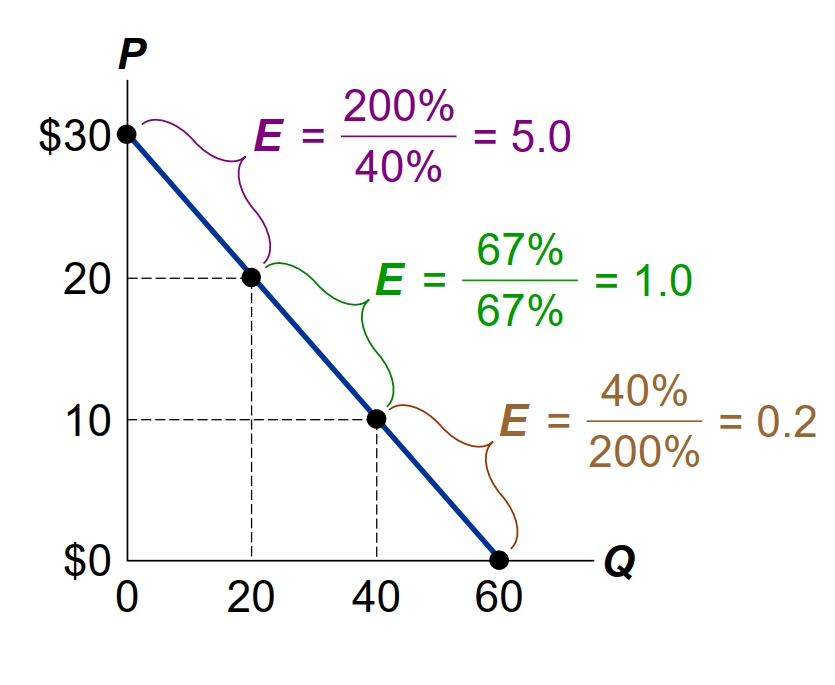
\includegraphics[width=0.6\textwidth]{线性需求曲线的弹性.png} % 插入图片,设置图片宽度为文本宽度的%
  \caption{线性需求曲线的弹性} % 为图片添加标题
\end{figure}

需求价格弹性与总收益:\\
\begin{figure}[H] 
  \centering % 使图片居中显示
  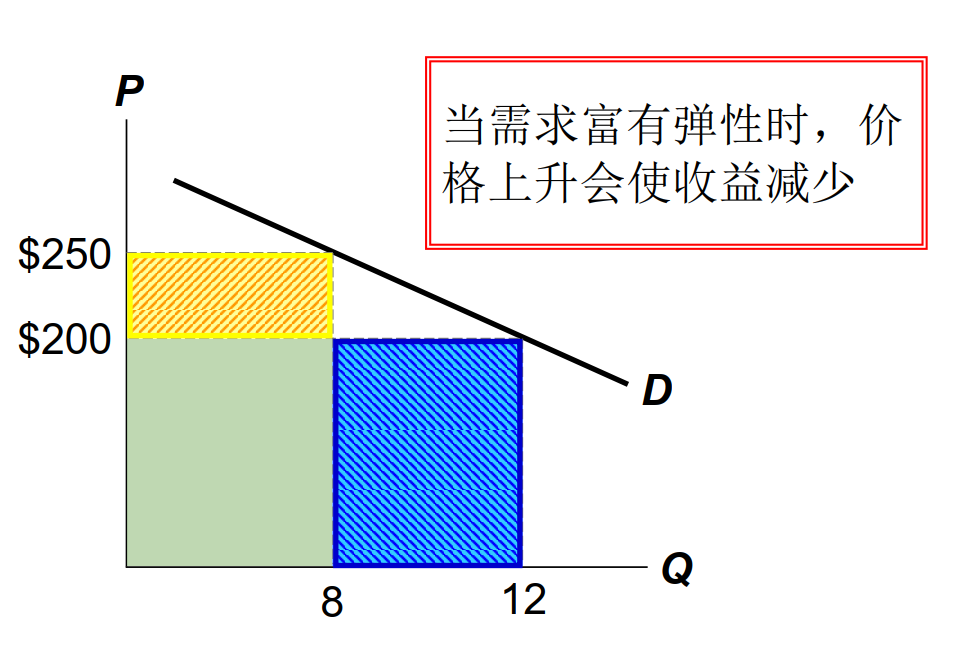
\includegraphics[width=0.5\textwidth]{弹性较大时的总收益变化.png} % 插入图片,设置图片宽度为文本宽度的%
  \caption{弹性较大时,价格上升,总收益减少} % 为图片添加标题
\end{figure}
\begin{figure}[H] 
  \centering % 使图片居中显示
  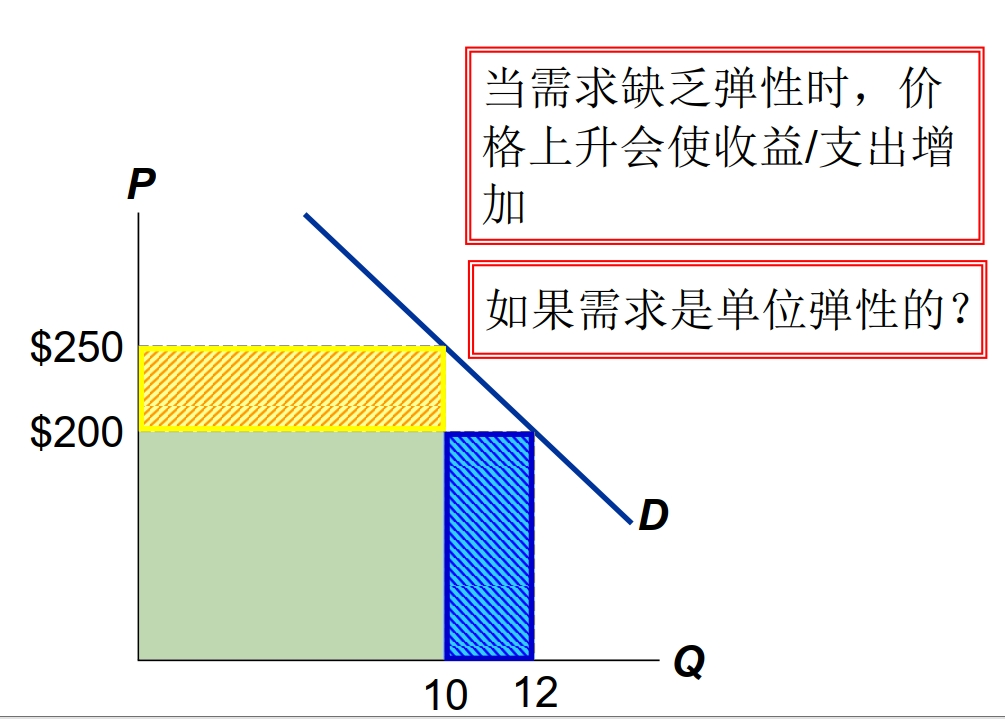
\includegraphics[width=0.5\textwidth]{弹性较小时的总收益变化.png} % 插入图片,设置图片宽度为文本宽度的%
  \caption{弹性较大时,价格上升,总收益增加} % 为图片添加标题
\end{figure}

其他需求弹性:\\

\textcolor{red}{需求收入弹性(income elasticity of demand)}:衡量消费者收入变动时需求量如何变动。正常物品的需求收入弹性为正数,而低档物品的为负数
$$E_{i} = \frac{\Delta Q / Q}{\Delta I / I}$$
$$E_{i} = \frac{dQ / Q}{dI / I}$$
\textcolor{red}{需求的交叉价格弹性}:替代品的交叉价格弹性为正数,互补品的交叉价格弹性为负数
$$E_{xy} = \frac{\Delta Q_x / Q_x}{\Delta P_y / P_y}$$
$$E_{xy} = \frac{dQ_x / Q_x}{dP_y / P_y}$$

%3.3.2供给价格弹性与供给曲线
\subsubsection{供给价格弹性与供给曲线}
\textcolor{red}{供给价格弹性(price elasticity of supply)}衡量供给量对价格变动的反应程度\\

\noindent 通过某一点的供给曲线越平坦,供给的价格弹性就越大\\
通过某一点的供给曲线越陡峭,供给的价格弹性就越小\\

供给价格弹性的决定因素:\\
\noindent1. 卖者调整物品生产量的灵活性\\
2. 长期供给的价格弹性都要大于短期供给的价格弹性

% Chapter 4

\section{税收与政府政策}
\subsection{价格控制}
\subsubsection{价格上限(price ceiling):出售一种物品或服务的法定最高价格}
价格上限是低于均衡价格的,是一种限制性约束,这导致了供给短缺
\begin{figure}[H] 
  \centering % 使图片居中显示
  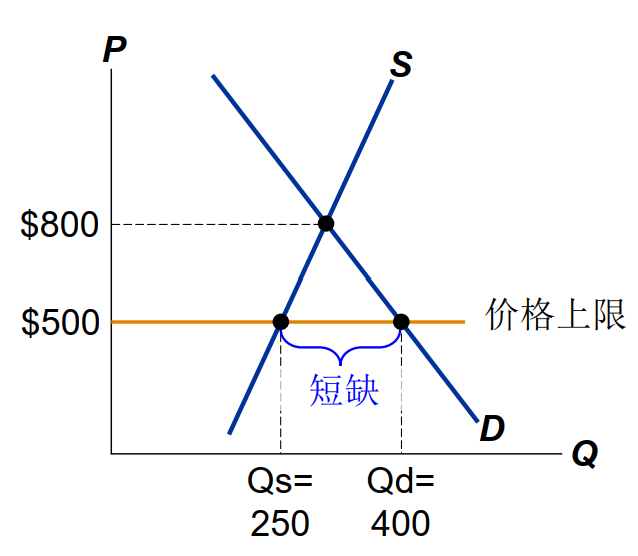
\includegraphics[width=0.4\textwidth]{价格上限.png} 
  \caption{价格上限} % 为图片添加标题
\end{figure}

\subsubsection{价格下限(price floor):出售一种物品或服务的法定最低价格}
e.g. 最低工资,粮食价格
价格上限是高于均衡价格的,此时价格下限引起了劳动力过剩=失业
\begin{figure}[H] 
  \centering % 使图片居中显示
  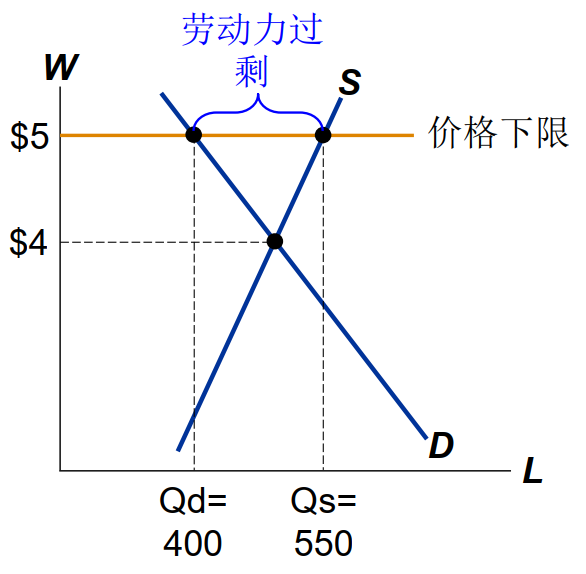
\includegraphics[width=0.4\textwidth]{价格下限.png} 
  \caption{价格下限} % 为图片添加标题
\end{figure}

\textcolor{red}{难点:价格下限与价格上限对市场的影响}


\newpage

\subsection{税收}
无论是对买者还是卖者征税,结果都一样。税收都在买者支付的价格和卖者得到的价格之间打入了一个楔子。提高了买者为该物品支付的价格,降低了卖者从该物品得到的价格,减少了购买与销售的数量。

\begin{figure}[H] 
  \centering % 使图片居中显示
  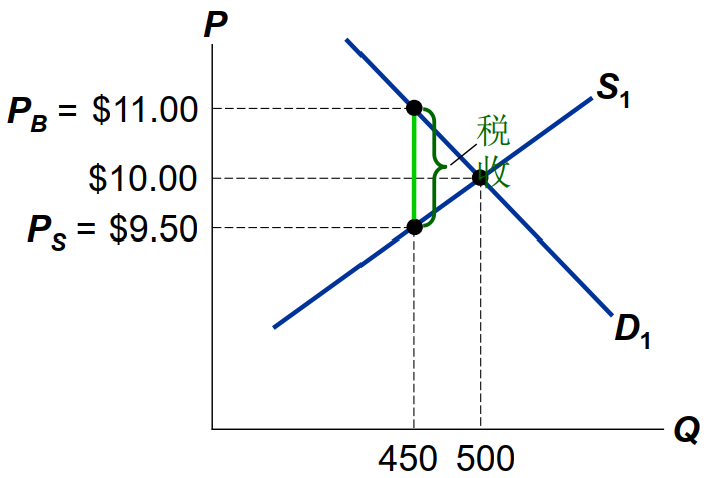
\includegraphics[width=0.4\textwidth]{税收.png} 
  \caption{税收} % 为图片添加标题
\end{figure}

练习题\\
假设某个市场可以由以下的供给和需求方程描述:\\
\[ Q_s=2P\]
\[ Q_d=300-P\]
a.假设对买者征收定额税T,新的需求曲线是什么?\\
b.新的市场均衡数量是多少?买者和卖者的税收负担是多少?\\

% a. 新的需求曲线
原需求方程为: 
\[Q_d = 300 - P\]

新的需求方程为: 
\[Q'_d = 300 - (P + T)\]

% b. 新的市场均衡数量及税收负担
为了找到新的市场均衡,我们设定供给等于需求:
\[Q_s = Q'_d\]
代入供给方程和新的需求方程:
\[2P = 300 - P - T\]
解这个方程可以找到新的均衡价格\(P_s^*=100 - \frac{T}{3}\)。\\

然后,将\(P^*\)代入任一方程式中(供给或需求)得到新的市场均衡数量\(Q^* = 200-\frac{2T}{3} = 300 - P_d\)。即\(P_d = 100 + \frac{2T}{3}\)。\\

税收负担可以通过比较税前后买家支付的价格和卖家接收的价格来确定。\\

税前均衡价格:
\[2P_0 = 300 - P_0\] 
\[P_0 = 100\]

得出卖者承担\(\frac{2T}{3}\), 卖者承担\(\frac{T}{3}\)






% Chapter 5

\section{福利经济学}
\textcolor{red}{福利经济学(welfare economics)}: 研究资源配置如何影响经济福利的一门学问\\

我们从考察买者和卖者的利益开始,然后考虑如何可以使所有人的利益最大化。最终我们将得出一个意义深远的结论: 市场上的供求均衡可以最大化买者和卖者的总利益 [市场通常是组织经济活动的一种好方法]
%5.1
\subsection{买者的利益:消费者剩余}
\textcolor{red}{支付意愿}:买者愿意为某种物品支付的最高金额,代表了买者对于该物品的评价(valuation)
\begin{figure}[H] 
  \centering % 使图片居中显示
  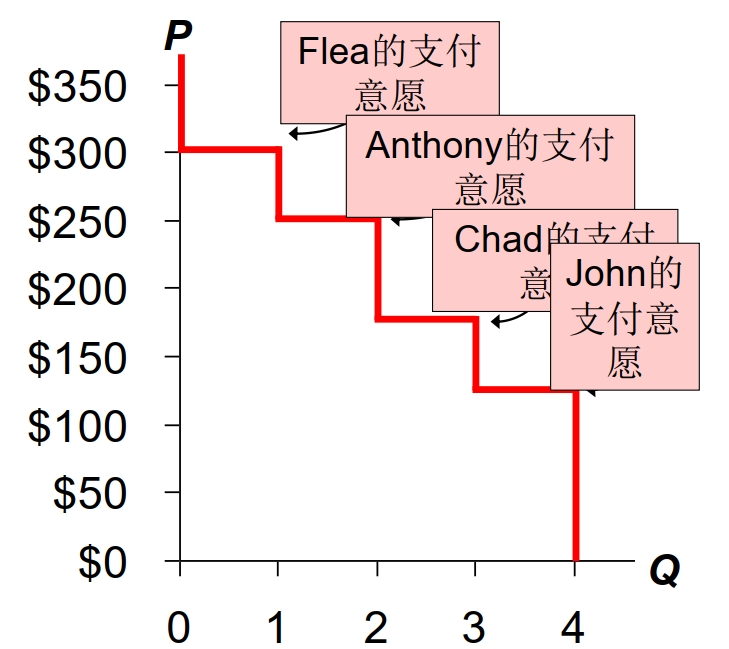
\includegraphics[width=0.4\textwidth]{支付意愿.png} 
  \caption{支付意愿} % 为图片添加标题
\end{figure}
在任意数量上,需求曲线的高度代表边界买者的支付意愿\\

\textcolor{red}{边际买者}:指如果价格再提高一点就首先离开市场的买者\\

\textcolor{red}{消费者剩余}:买者愿意为一种物品支付的量减去其为此实际支付的量。
\[
\text{消费者剩余} = \int_{P}^{P_{\text{最大}}} D(P) \, dP - Q \cdot P
\]
\indent\textcolor{red}{总消费者剩余}:所有消费者剩余之和。等于需求曲线以下,价格之上的面积。
\[
\text{总消费者剩余} = \int_{0}^{Q} P_{\text{d}}(q) \, dq - P \cdot Q
\]
\begin{figure}[H] 
  \centering % 使图片居中显示
  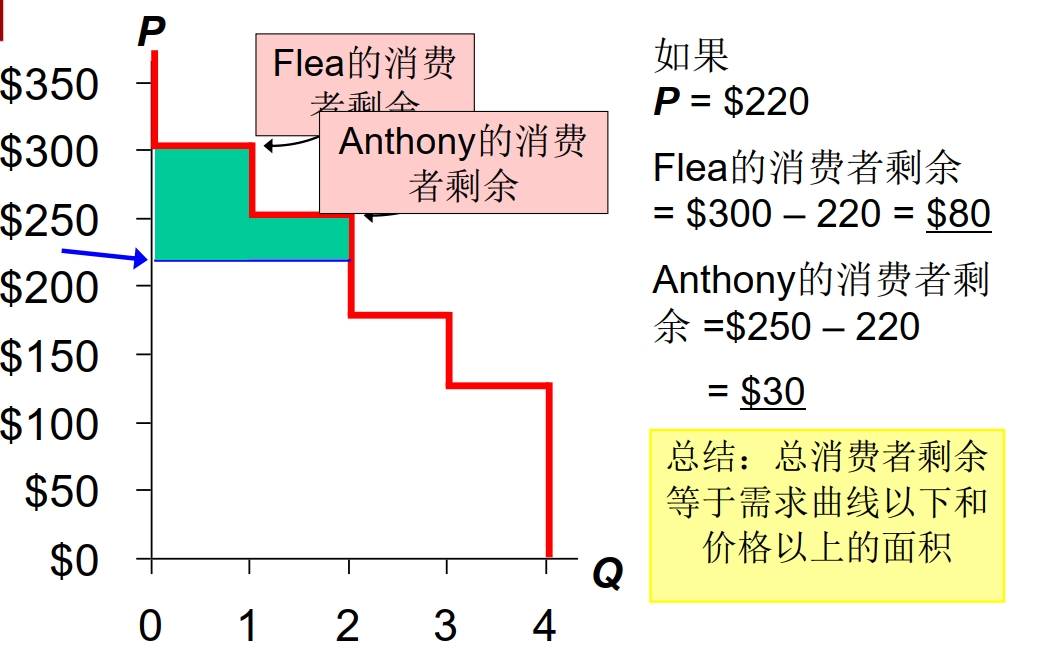
\includegraphics[width=0.6\textwidth]{消费者剩余.png} 
  \caption{消费者剩余} % 为图片添加标题
\end{figure}
大量买者的需求曲线与消费者剩余\\
\begin{figure}[H] 
  \centering % 使图片居中显示
  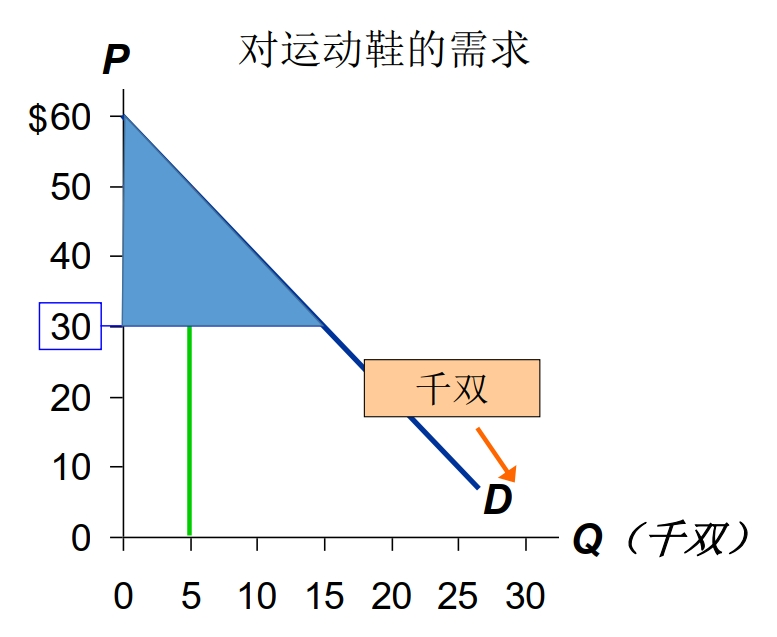
\includegraphics[width=0.4\textwidth]{大量买者的消费者剩余.png} 
  \caption{大量买者的消费者剩余} % 为图片添加标题
\end{figure}
\[
S = \frac{1}{2} \times (15 - 0) \times (60 - 30)
\]

更高的价格会减少消费者剩余\\
\begin{figure}[H] 
  \centering % 使图片居中显示
  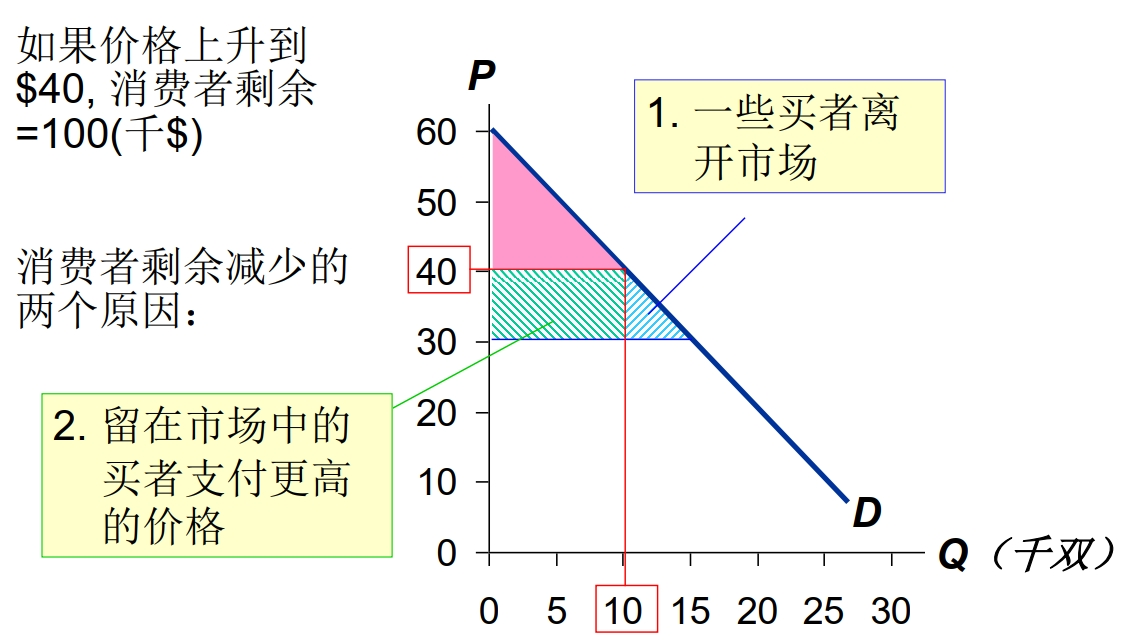
\includegraphics[width=0.6\textwidth]{更高的价格会减少消费者剩余.png} 
  \caption{更高的价格会减少消费者剩余} % 为图片添加标题
\end{figure}

%5.2
\subsection{卖者的利益:生产者剩余}

\textcolor{red}{成本(cost)}: 卖者为了生产一种物品而必须放弃的所有东西的价值。其实就是机会成本: 包括所有用于生产物品的资源的成本和卖者对于他们自己时间、精力的评价。一个卖者生产和出售物品或服务,除非价格高于他或她的成本。因此,成本衡量了出售意愿。\\

\subsubsection{成本与供给曲线}
\begin{figure}[H] 
  \centering % 使图片居中显示
  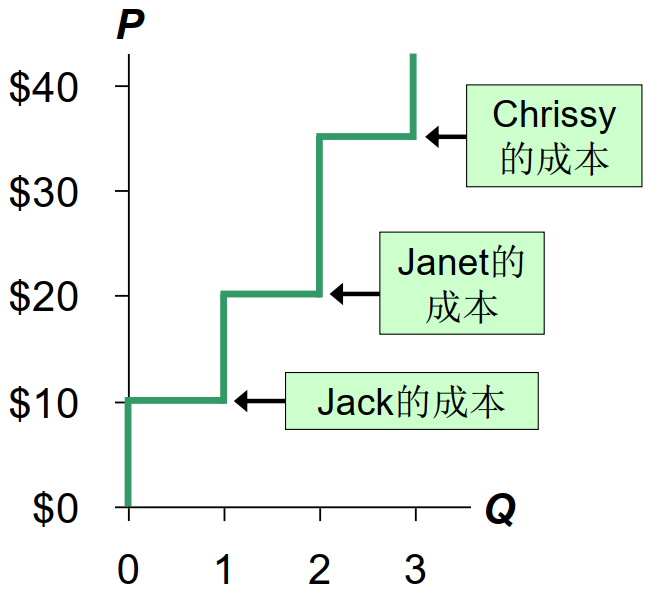
\includegraphics[width=0.4\textwidth]{成本与供给曲线.png} 
  \caption{成本与供给曲线} % 为图片添加标题
\end{figure}

\noindent 在每个数量,供给曲线的高度是边际卖者的成本。\\
\textcolor{red}{边际卖者}:如果价格再低一点就首先离开市场的卖者

\subsubsection{生产者剩余与供给曲线}

\noindent \textcolor{red}{生产者剩余(producer surplus)}:出售价格减去其生产成本\\
生产者剩余 = 价格 - 成本\\
总生产者剩余等于价格以下和供给曲线以上的面积\\

\begin{figure}[H] 
  \centering % 使图片居中显示
  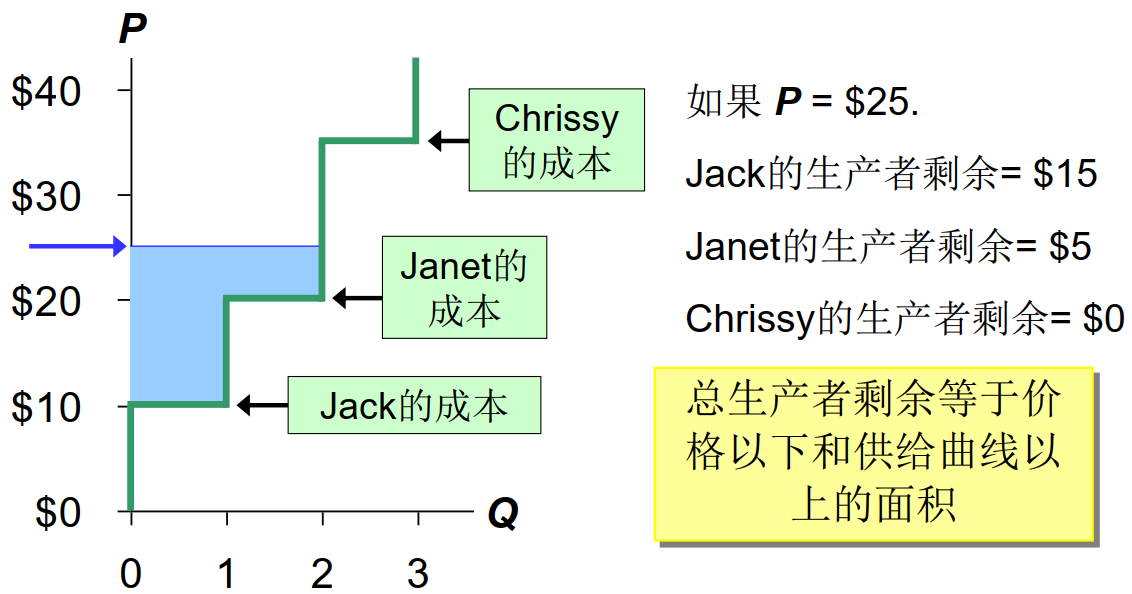
\includegraphics[width=0.6\textwidth]{生产者剩余与供给曲线.png} 
  \caption{生产者剩余与供给曲线} % 为图片添加标题
\end{figure}
大量卖者的生产者剩余
\begin{figure}[H] 
  \centering % 使图片居中显示
  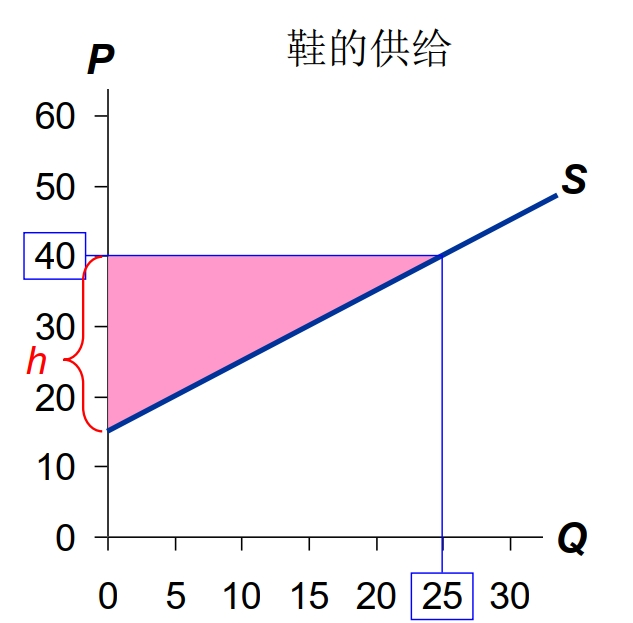
\includegraphics[width=0.4\textwidth]{大量卖者的生产者剩余.png} 
  \caption{大量卖者的生产者剩余} % 为图片添加标题
\end{figure}
\textcolor{red}{总生产者剩余}:所有生产者剩余之和。等于需求曲线以上,价格以下的面积。
\[
S = \frac{1}{2} \times (25 - 0) \times (40 - 15)
\]

更低的价格将减少生产者剩余\\
\begin{figure}[H] 
  \centering % 使图片居中显示
  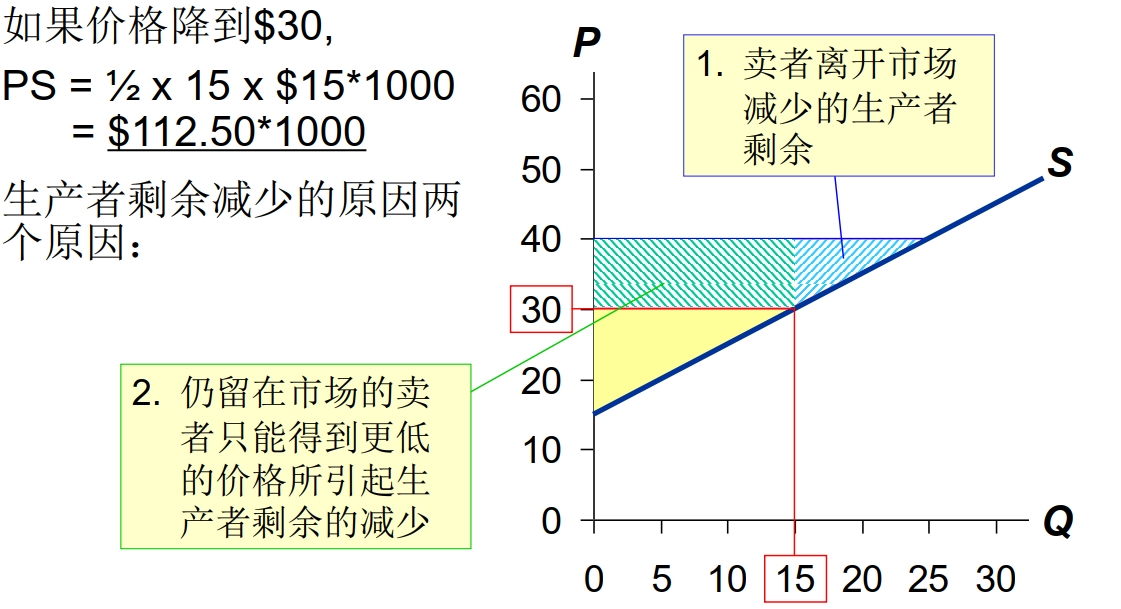
\includegraphics[width=0.6\textwidth]{更低价格的生产者剩余.png} 
  \caption{更低价格的生产者剩余} % 为图片添加标题
\end{figure}

%5.3
\subsection{市场效率(市场总福利)}
市场总剩余(总福利) = CS (consumer supply) +  PS (producer supply)  =  (买者的评价) – (买者支付的量) + (卖者得到的量) – (卖者的成本) =  (买者的评价) – (卖者的成本) = (买者+卖者)参与市场贸易得到的总收益\\

如果资源配置使总剩余最大化,那我们可以说,这种配置是有效率的。\\
\begin{figure}[H] 
  \centering % 使图片居中显示
  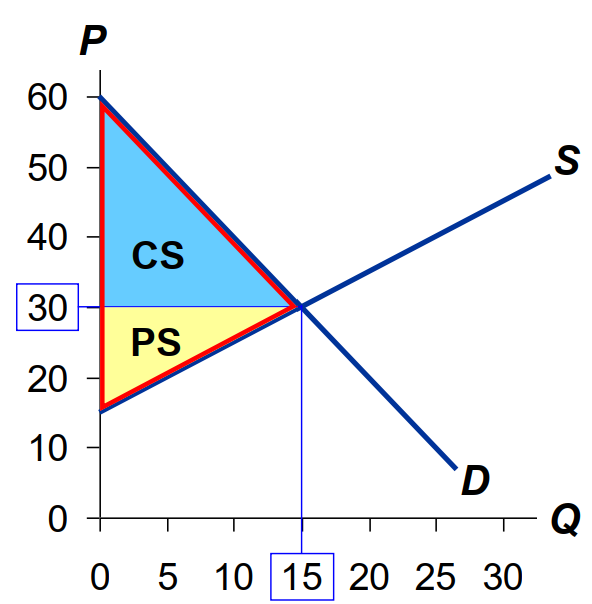
\includegraphics[width=0.4\textwidth]{市场总福利.png} 
  \caption{市场均衡时的市场总福利} % 为图片添加标题
\end{figure}
当市场均衡时,市场总剩余最大(左侧图形面积最大);高于均衡的数量会使总剩余减少(左侧面积 - 右侧面积);低于均衡的数量会使总剩余减少(左侧面积比均衡时的三角形面积小)。\\

市场均衡配置是最有效的配置。市场均衡产量使总剩余最大:在其他任何数量下,向市场均衡数量移动都能使总剩余增加。

\subsection{税收的代价}
\begin{figure}[H] 
  \centering % 使图片居中显示
  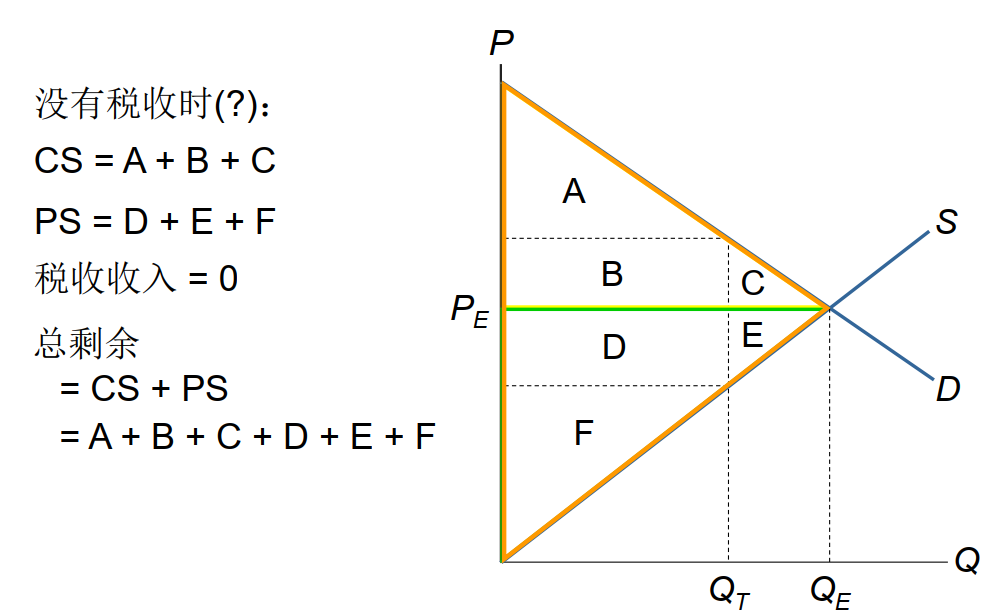
\includegraphics[width=0.6\textwidth]{没有税收时的总福利.png} 
  \caption{没有税收时的总福利} % 为图片添加标题
\end{figure}
\begin{figure}[H] 
  \centering % 使图片居中显示
  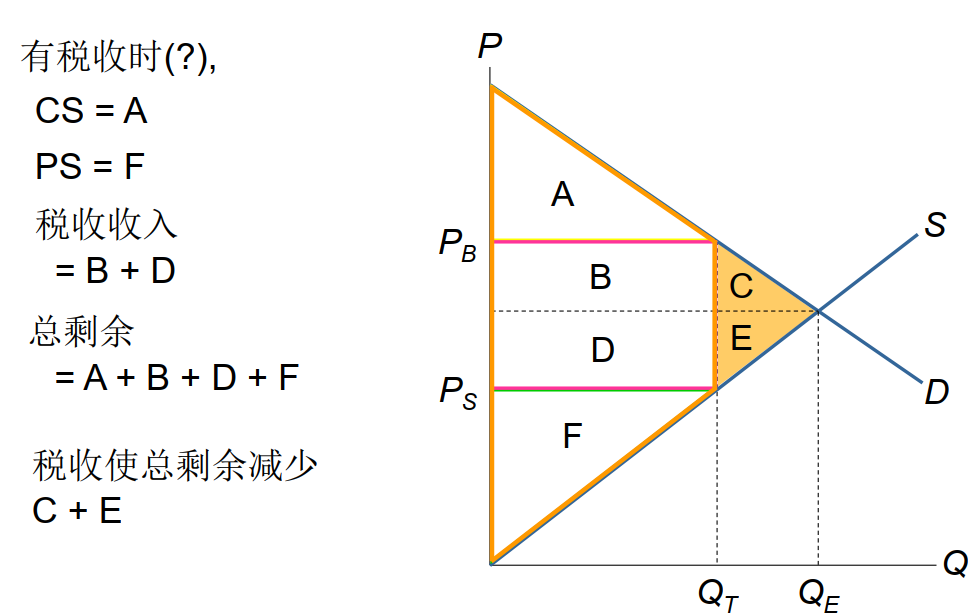
\includegraphics[width=0.6\textwidth]{有税收时的总福利.png} 
  \caption{有税收时的总福利} % 为图片添加标题
\end{figure}

C + E 被称为税收的\textcolor{red}{无谓损失 (deadweight loss)}: 市场扭曲(例如税收)引起总剩余减少的部分。由于税收,在QT 与 QE 单位之间的物品没有被售出。\\

决定无谓损失大小的因素:弹性。弹性越小,无谓损失越小。\\

\begin{figure}[H] 
  \centering % 使图片居中显示
  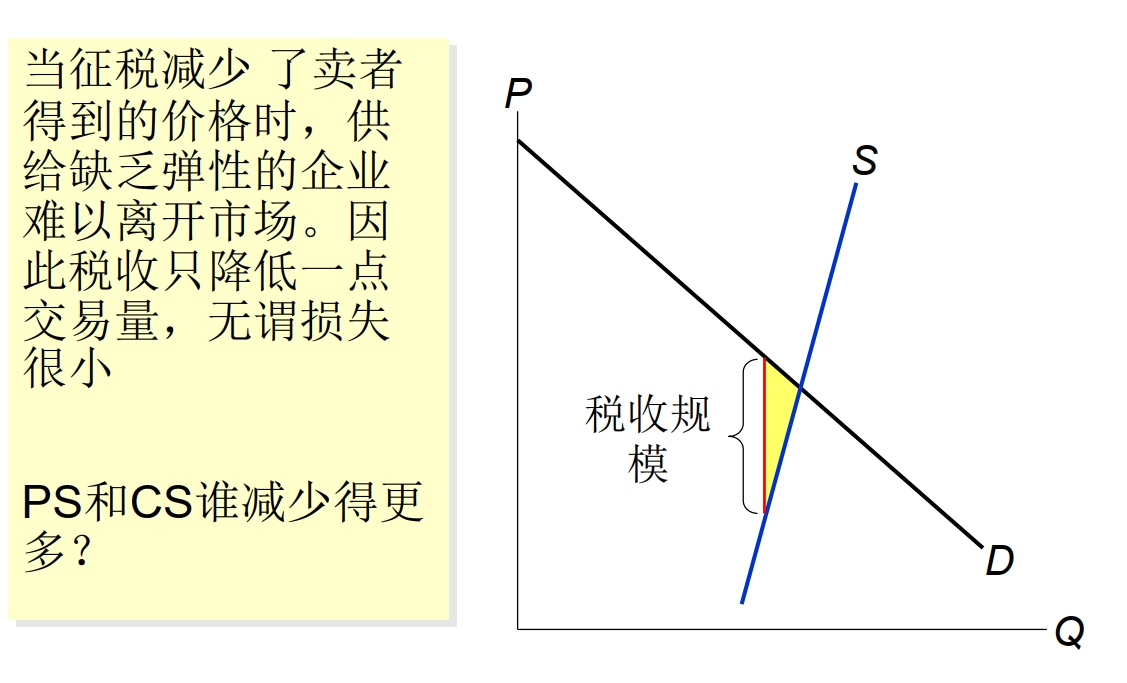
\includegraphics[width=0.5\textwidth]{弹性小,无谓损失小.png} 
  \caption{弹性小,无谓损失小} % 为图片添加标题
\end{figure}
\begin{figure}[H] 
  \centering % 使图片居中显示
  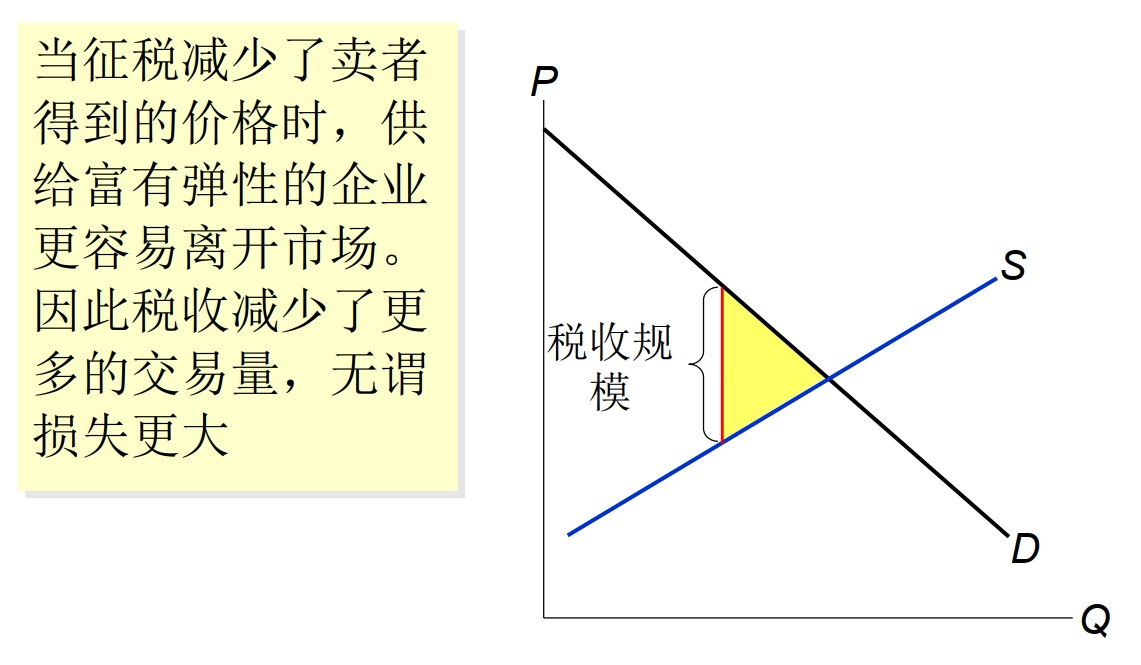
\includegraphics[width=0.5\textwidth]{弹性大,无谓损失大.png} 
  \caption{弹性大,无谓损失大} % 为图片添加标题
\end{figure}

税收规模增长速度比无谓损失的增长速度小
\begin{figure}[H] 
  \centering % 使图片居中显示
  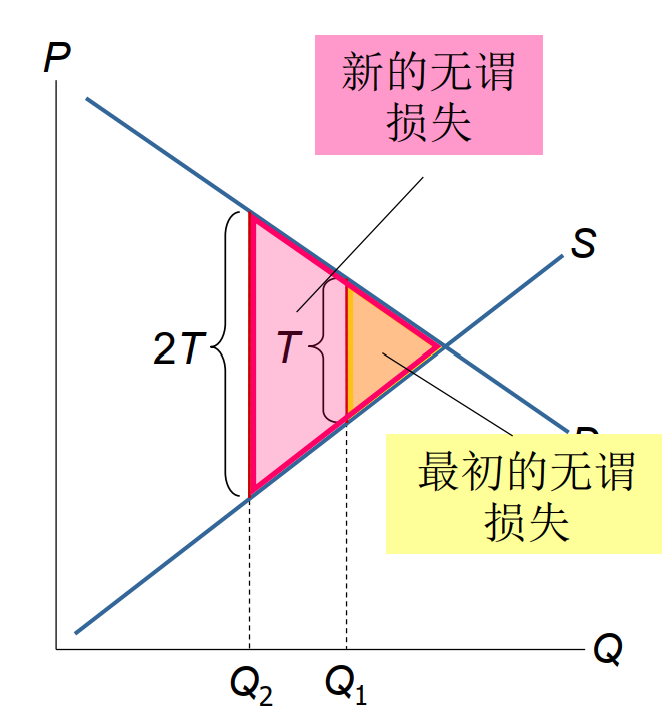
\includegraphics[width=0.4\textwidth]{税收规模与无谓损失.png} 
  \caption{税收规模增长速度比无谓损失的增长速度小} % 为图片添加标题
\end{figure}

含义:当税率低时,提高或降低税率既不会带来太大的损失,也不会带来太多的好处;当税率高时,提高税率的损失非常大,而降低税率的好处也非常明显
\begin{figure}[H] 
  \centering % 使图片居中显示
  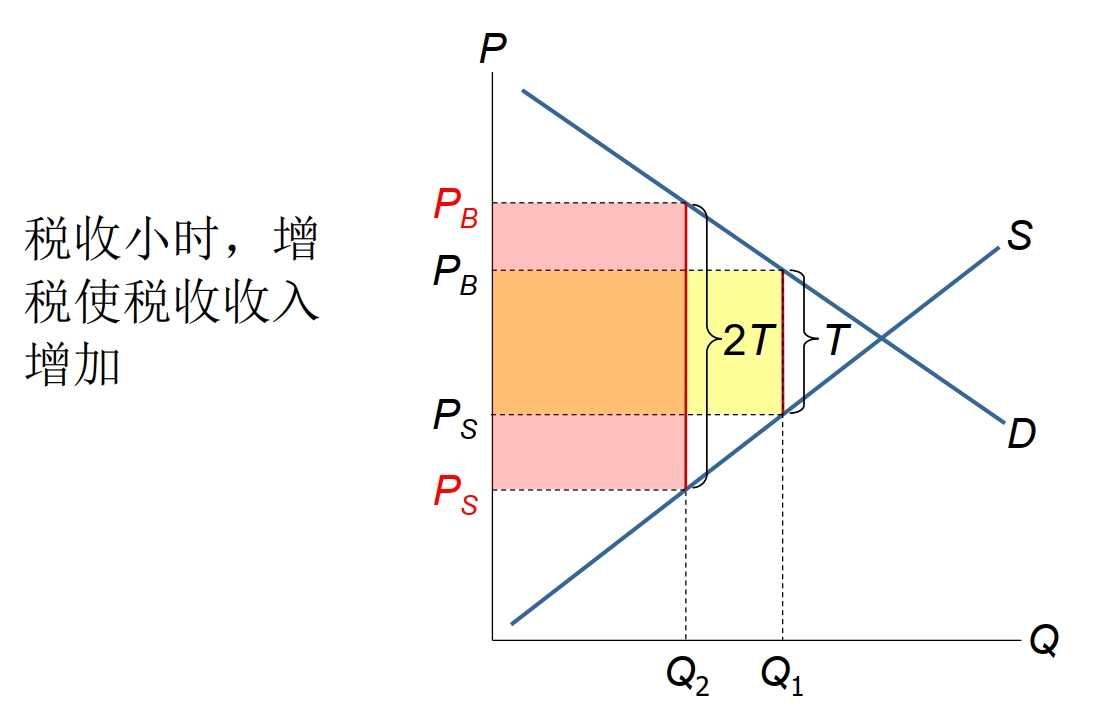
\includegraphics[width=0.5\textwidth]{税收小.png} 
  \caption{税收小,增税使税收收入增加} % 为图片添加标题
\end{figure}
\begin{figure}[H] 
  \centering % 使图片居中显示
  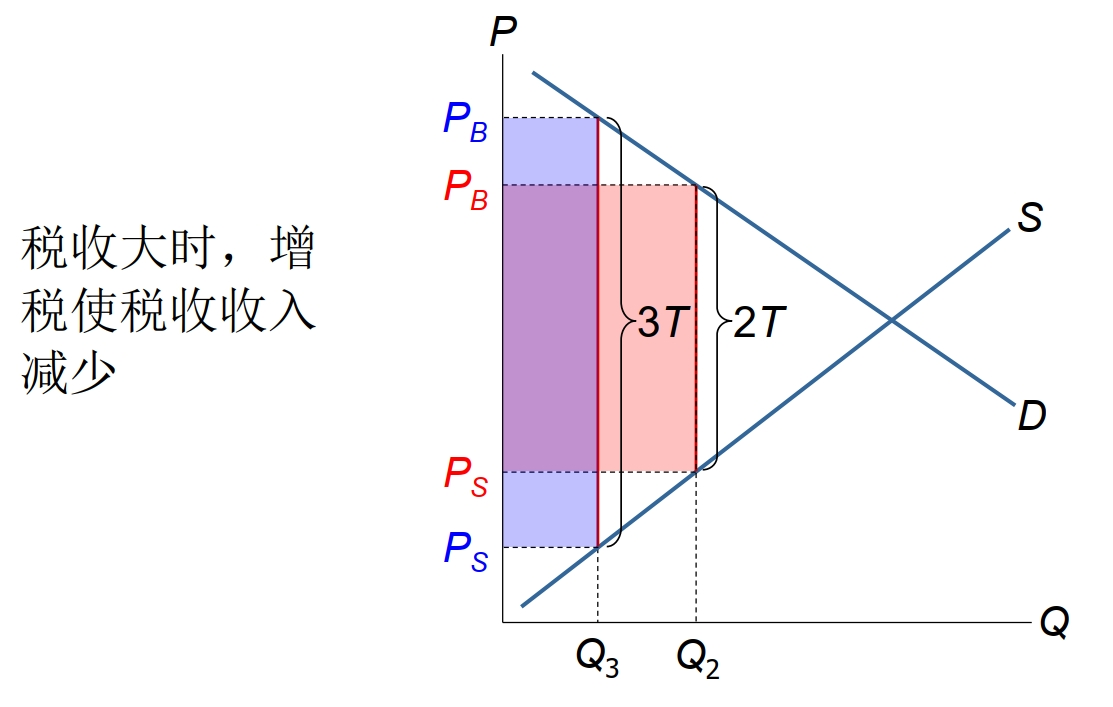
\includegraphics[width=0.5\textwidth]{税收大.png} 
  \caption{税收大,增税使税收收入减少} % 为图片添加标题
\end{figure}
\begin{figure}[H] 
  \centering % 使图片居中显示
  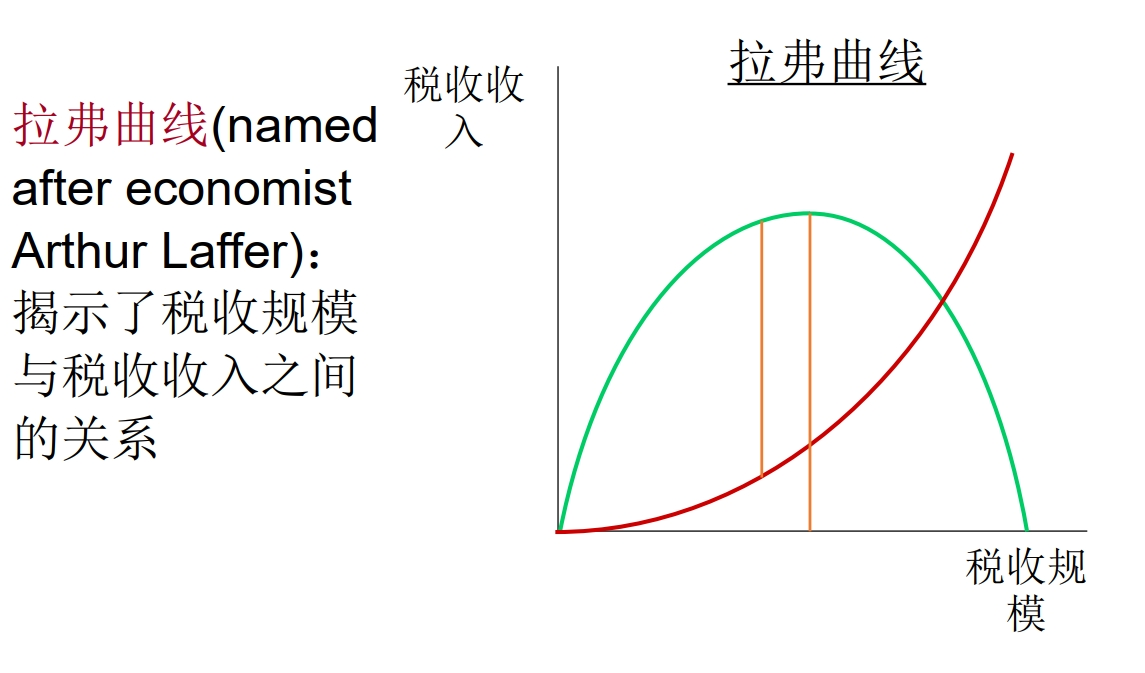
\includegraphics[width=0.5\textwidth]{拉弗曲线.png} 
  \caption{拉弗曲线} % 为图片添加标题
\end{figure}

\newpage
%Chapter 6外部性
\section{外部性} 

% 6.1
\subsection{外部性和市场无效率}
\textcolor{red}{外部性}:一个人的行为对旁观者福利的无补偿的影响\\
外部性有负外部性或正外部性之分,这取决于对旁观者福利的影响是有利的还是不利的。\\

\noindent 存在负外部性:市场均衡数量大于社会合意的数量\\
存在正外部性:市场均衡的数量小于社会合意的数量\\

\noindent 为了解决问题,可以使外部性内在化,使价格=社会成本。\\
对负外部性的物品征税,对正外部性的物品补贴\\

%6.1.1负外部性
\subsubsection{负外部性}
对旁观者福利的影响是不利的。e.g. 污染 (煤炭生产将排放污染物 → 损害周围居民的健康)\\

\textcolor{red}{社会成本} = 生产者私人成本+受到污染的不利影响的旁观者的成本\\

负外部性的社会成本在供给曲线(生产者私人成本)上方
\begin{figure}[H] 
  \centering % 使图片居中显示
  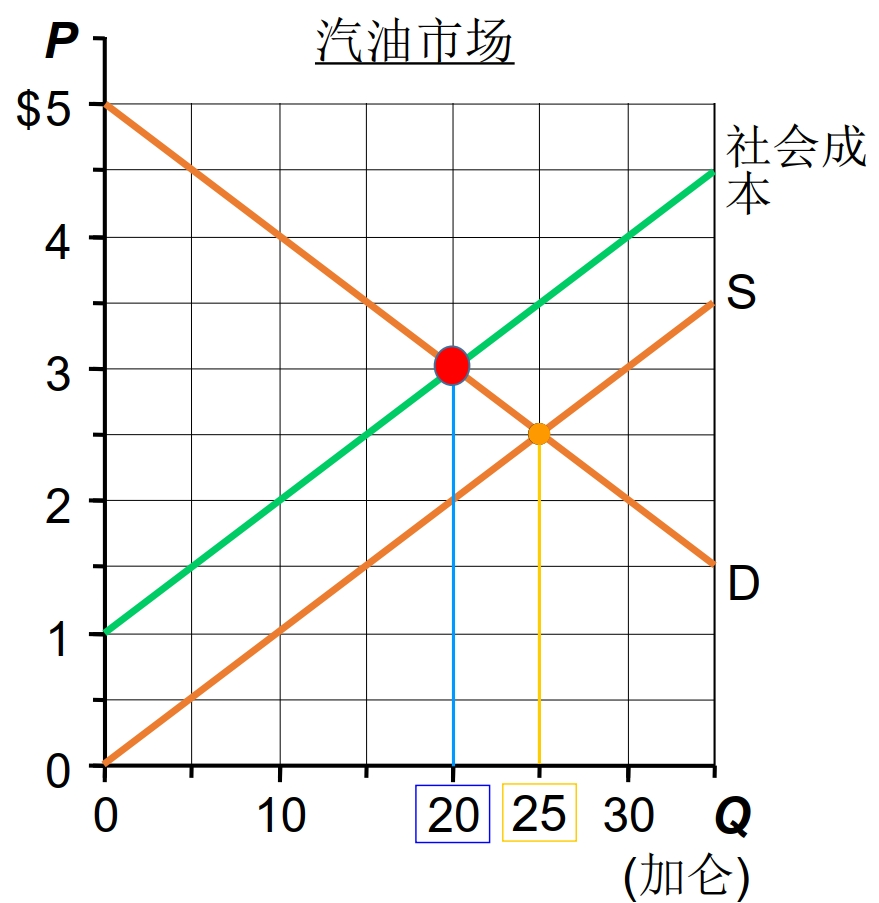
\includegraphics[width=0.4\textwidth]{负外部性.png} 
  \caption{负外部性的社会成本} % 为图片添加标题
\end{figure}
在有负外部性的情况下,市场总剩余并不是最大(最佳均衡点右侧的三角形面积是无谓损失(成本>价值)),最佳生产量应当小于市场均衡量。\\

\textcolor{red}{外部性内在化}:改变激励,以使人们考虑到自己行为的外部效应。例如对卖者征税,使卖者成本=社会成本。\\

当市场参与者必须支付社会成本时,市场均衡= 社会均衡

%6.1.2正外部性
\subsubsection{正外部性}
\noindent 对旁观者福利的影响是有利的。e.g. 个人的教育\\
社会价值 = 私人价值+教育为旁观者带来的有利影响的价值\\
\begin{figure}[H] 
  \centering % 使图片居中显示
  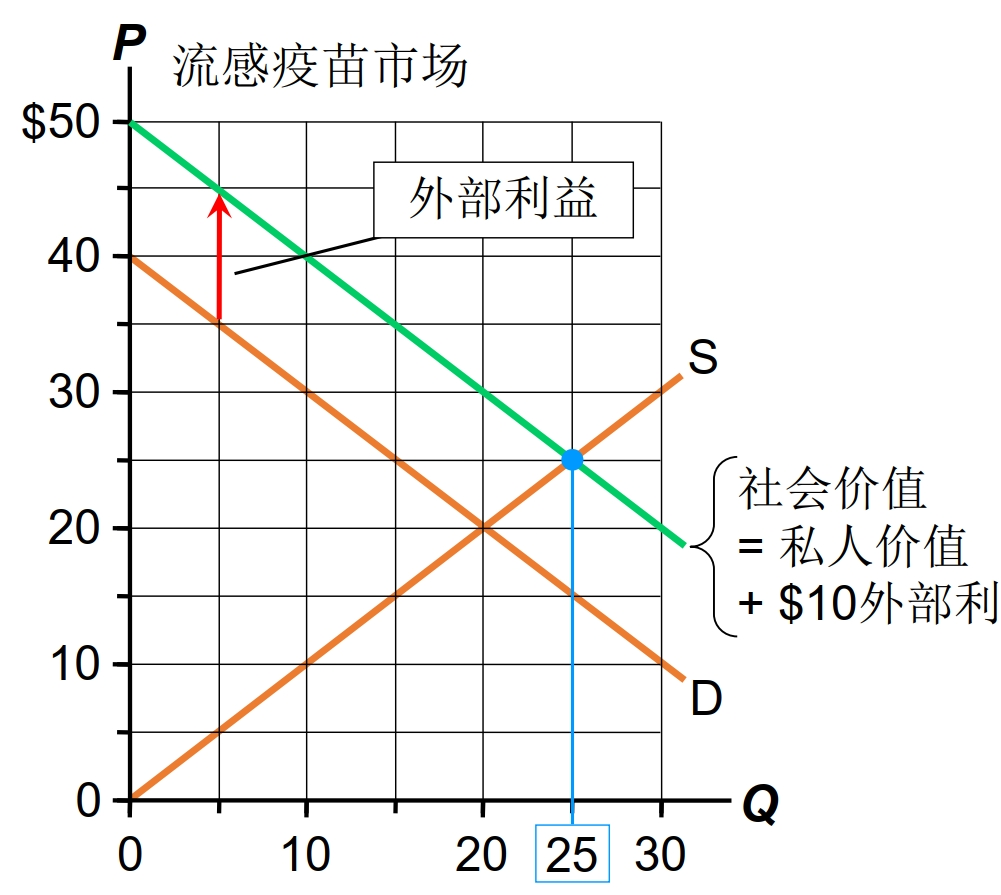
\includegraphics[width=0.4\textwidth]{正外部性.png} 
  \caption{正外部性的社会成本} % 为图片添加标题
\end{figure}

%6.2
\subsection{针对外部性的政府解决方法}
%6.2.1
\subsubsection{命令与控制政策:直接管制}
\noindent 例如:\\
• 限制排放的污染数量\\
• 强制企业采取某种技术来减少排放量:e.g. 限制每单位产出的排污量
%6.2.2
\subsubsection{以市场为基础的政策 (market based)}
向私人决策者提供激励,然后市场会自动矫正到最优数量\\

\textbf{A. 矫正性税收与补贴}\\

矫正税, 也被称为庇古税。理想的矫正税= 外部成本;理想的矫正补贴=外部利益\\

\textcolor{red}{难点:施加庇古税为什么可以做到没有无谓损失?}\\

矫正市场价格:矫正税通过增加生产成本,使得市场价格更加真实地反映了商品或服务的社会成本。这导致价格上升,从而减少了对具有负外部性商品或服务的需求,使得生产量降低到社会最优水平。\\


\noindent • 矫正税和其他税的影响不同:\\

其他税收与补贴会扭曲激励,并使经济远离社会最优数量。\\

而矫正性税收与补贴:\\
1. 使私人激励与社会的利益结合在一起\\
2. 使私人决策者做决策时考虑到他们行为的外部利益与外部成本\\
3. 使经济向一个资源配置更有效率的方向移动\\

矫正税/补贴的难点:外部成本与外部利益非常难以测量,很难说政府的税收和补贴究竟是否合理\\

\textbf{B. 可交易的污染许可证 (tradable permit) }\\

\noindent 关键假设:企业的减排成本不同\\

在市场均衡里,减排成本低的企业会减排,并出售他们的permit;减排成本高的企业更有动机买permit(前提是permit)的价格低于减排成本。\\


% 6.3 公共物品与公共资源
私人物品的特点:排他性(可以阻止一些人使用这个物品的特性)\&竞争性(一个人使用该物品将减少其他人对它的使用的特性)\\

\textcolor{red}{公共物品(public goods)}:即无排他性又无竞争性的物品\\

公共物品由于搭便车问题,个人没有动机去提供,所以必须依靠政府\\

\textcolor{red}{公共资源(public resources)}:没有排他性但具有竞争性的物品\\

公共资源的使用具有负外部性,政府可以通过管制,税收能政策来解决公地悲剧,但更好的办法可能是确定产权(将公共资源转化为私人产权)

\newpage
%Chapter 7
\section{生产成本}

%7.1
\setstretch{1.5}
\subsection{生产与成本}
%7.1.1
\subsubsection{成本}
成本=显性成本+隐性成本\\
\textcolor{red}{显性成本}:需要企业支出货币的投入成本。例如:支付给工人的工资。\\
\textcolor{red}{隐性成本}:不需要企业支付货币的投入成本。例如:企业所有者时间的机会成本。\\
经济利润与会计利润:\\
\begin{figure}[H] 
  \centering % 使图片居中显示
  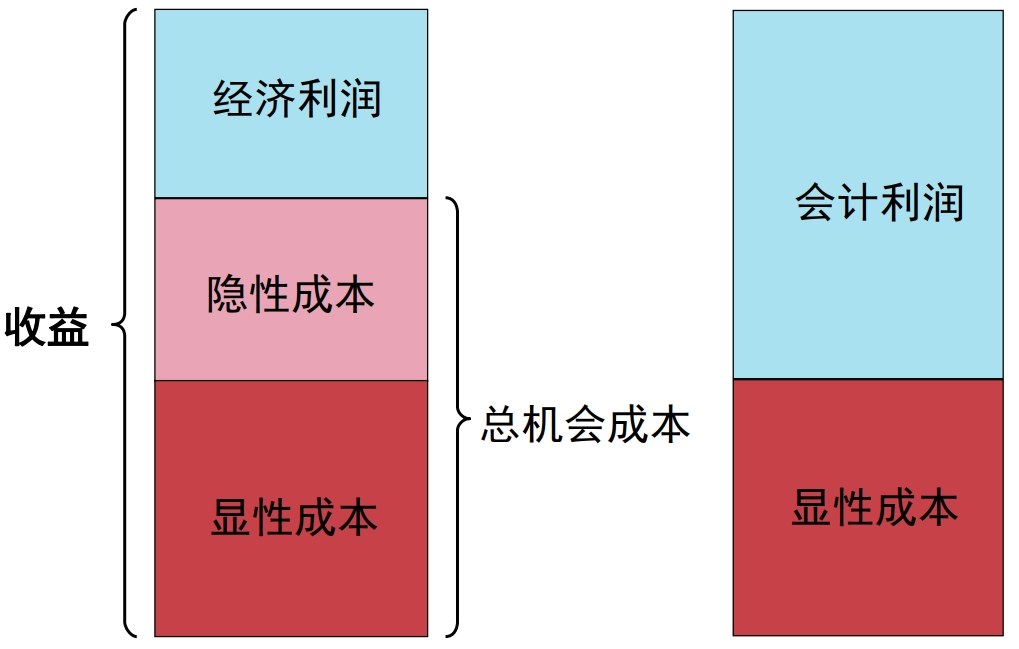
\includegraphics[width=0.4\textwidth]{经济利润与会计利润.png} 
  \caption{经济利润与会计利润} % 为图片添加标题
\end{figure}
%7.1.2
\subsubsection{生产函数}
\textcolor{red}{生产函数}: 用于生产一种物品的投入量与该物品产量(Q)之间的关系\\

\textcolor{red}{投入量(input)}:劳动力L+资本K\\
L: 劳动的时间,劳动的人数; K: 例如机器,厂房,土地
\[
Q=f(L,K)
\]
Q的上限由K决定\\

投入量可分为\textcolor{red}{可变投入量(variable input)}和\textcolor{red}{固定投入量(fixed input)},前者容易改变(例如劳动时间),后者不容易改变(例如厂房的大小)\\
\begin{figure}[H] 
  \centering % 使图片居中显示
  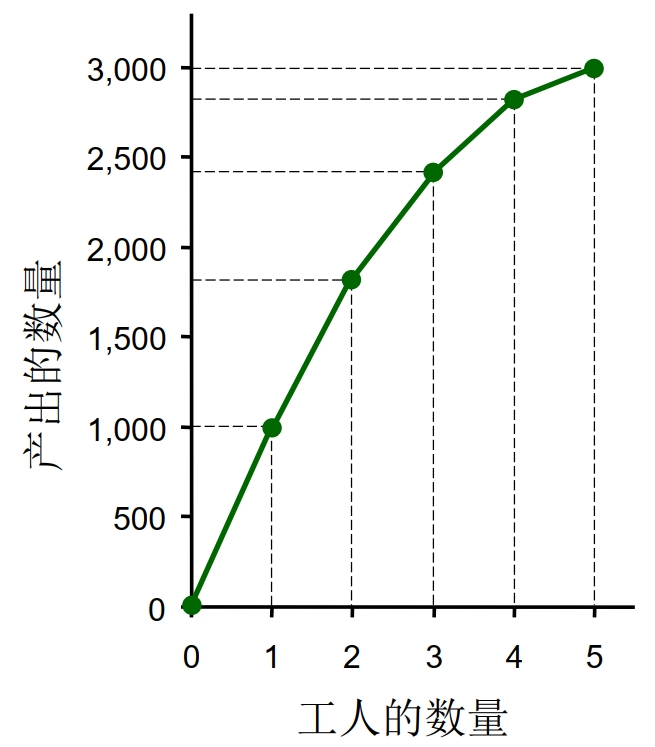
\includegraphics[width=0.4\textwidth]{生产函数.png} 
  \caption{生产函数:越来越平坦(边际收益递减)} % 为图片添加标题
\end{figure}

\textcolor{red}{投入的边际产量}:在其他投入量不变情况下,增加一单位投入所引起的产量增加\\

∆Q = 产出的变动量, ∆L = 劳动的变动量
\textcolor{red}{劳动的边际产量:(生产函数的斜率)}
\[
(MP_L) = \frac{\Delta Q}{\Delta L}
\]
%7.2
\subsection{成本的衡量指标}

\noindent 总成本(TC: total costs)分为:\\
\textcolor{red}{固定成本(FC: fixed costs)}:不随着产量变动而变动的成本\\
e.g.设备成本,偿还贷款,租金支付 - 固定投入带来的成本\\
\textcolor{red}{可变成本(VC: variable costs)}:随着产量变动而变动的成本\\
e.g.支付给工人的工资,原材料的成本 - 可变投入带来的成本\\

\begin{figure}[H] 
  \centering % 使图片居中显示
  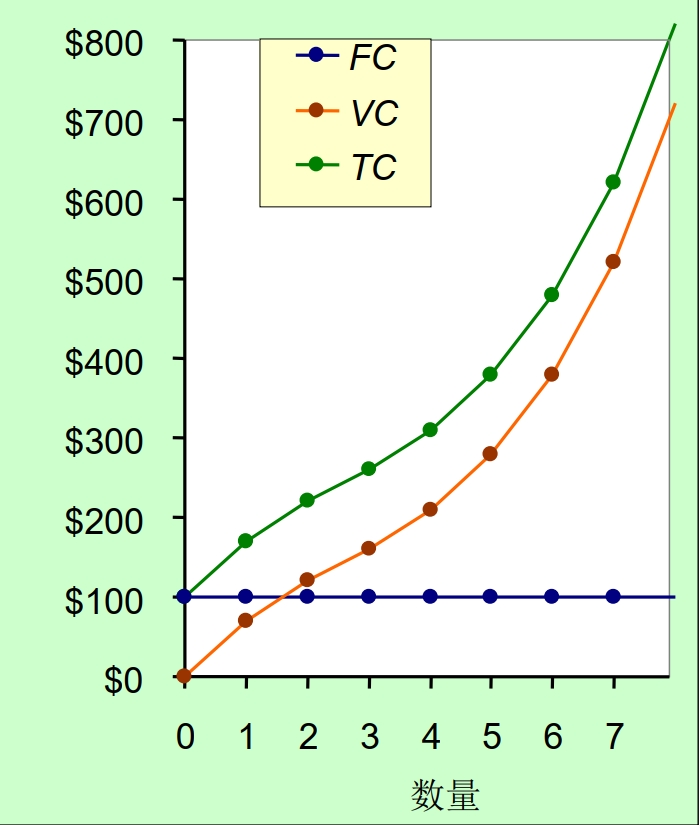
\includegraphics[width=0.3\textwidth]{成本函数.png} 
  \caption{TC, FC, VC} % 为图片添加标题
\end{figure}

\textcolor{red}{边际成本(MC: marginal costs)}:额外一单位产量所引起的总成本的增加\\
\[
(MC) = \frac{\Delta TC}{\Delta Q} = \frac{\Delta VC}{\Delta Q} 
\]
边际成本是边际产量的倒数,边际成本递增(斜率可以不变,也可以递增)\\

\textcolor{red}{平均总成本(ATC)}:平均固定成本(AFC)+平均可变成本(AVC)
\indent 告诉我们总成本在所生产的所有单位中平均分摊,平均一单位产品的成本。
\[
ATC = \frac{TC}{Q} = AFC + AVC
\]
\begin{figure}[H] 
  \centering % 使图片居中显示
  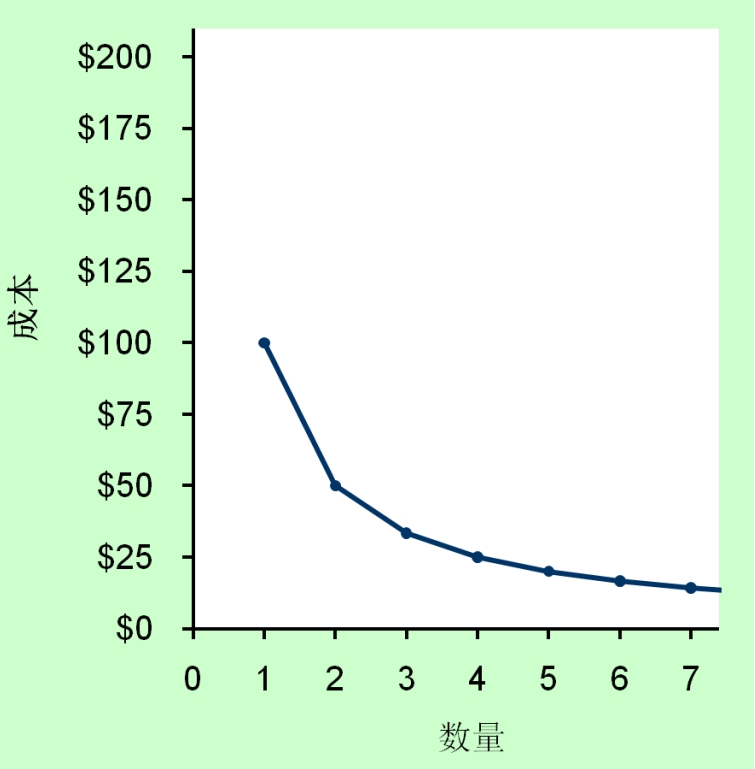
\includegraphics[width=0.4\textwidth]{AFC.png} 
  \caption{平均固定成本(AFC)} % 为图片添加标题
\end{figure}
\begin{figure}[H] 
  \centering % 使图片居中显示
  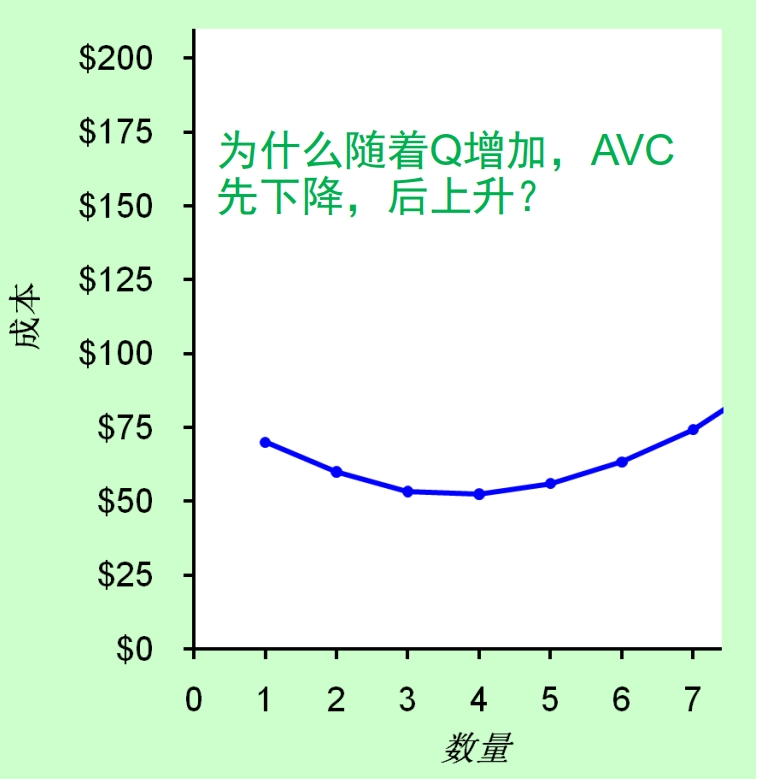
\includegraphics[width=0.4\textwidth]{AVC.png} 
  \caption{平均可变成本(AVC)} % 为图片添加标题
\end{figure}
随着Q增加,AVC先下降,后上升

\begin{figure}[H] 
  \centering % 使图片居中显示
  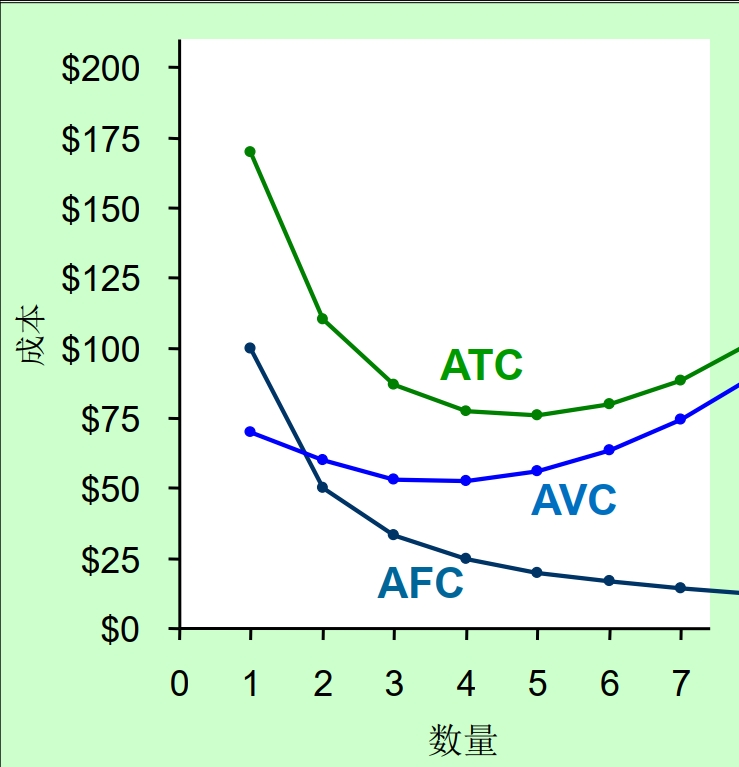
\includegraphics[width=0.4\textwidth]{ATC.png} 
  \caption{平均总成本(ATC):U形} % 为图片添加标题
\end{figure}
平均总成本曲线是U形。U形曲线的低端是企业的有效规模(efficient scale)——使ATC最小的产量\\

\begin{figure}[H] 
  \centering % 使图片居中显示
  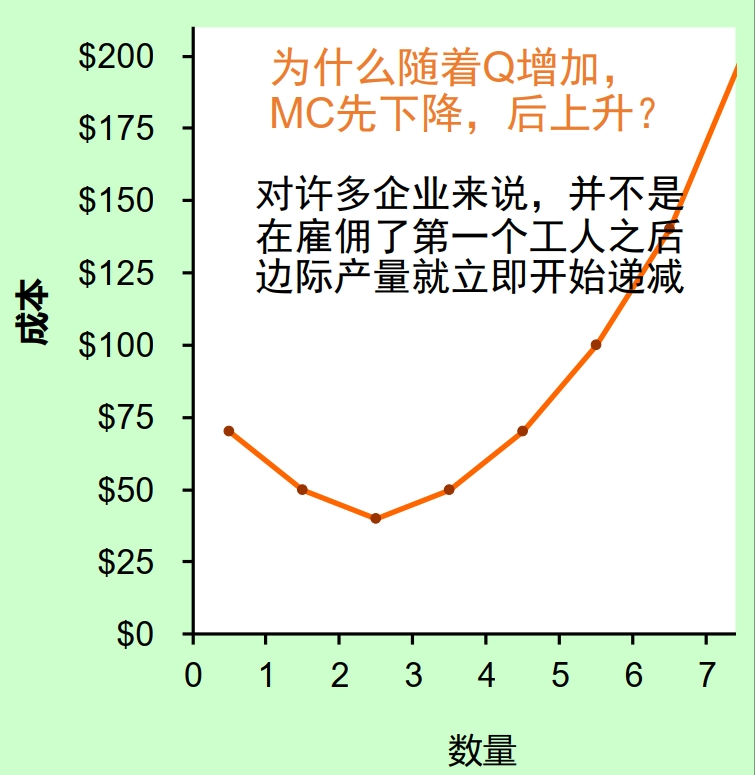
\includegraphics[width=0.4\textwidth]{MC.png} 
  \caption{边际成本(MC)} % 为图片添加标题
\end{figure}

\begin{figure}[H] 
  \centering % 使图片居中显示
  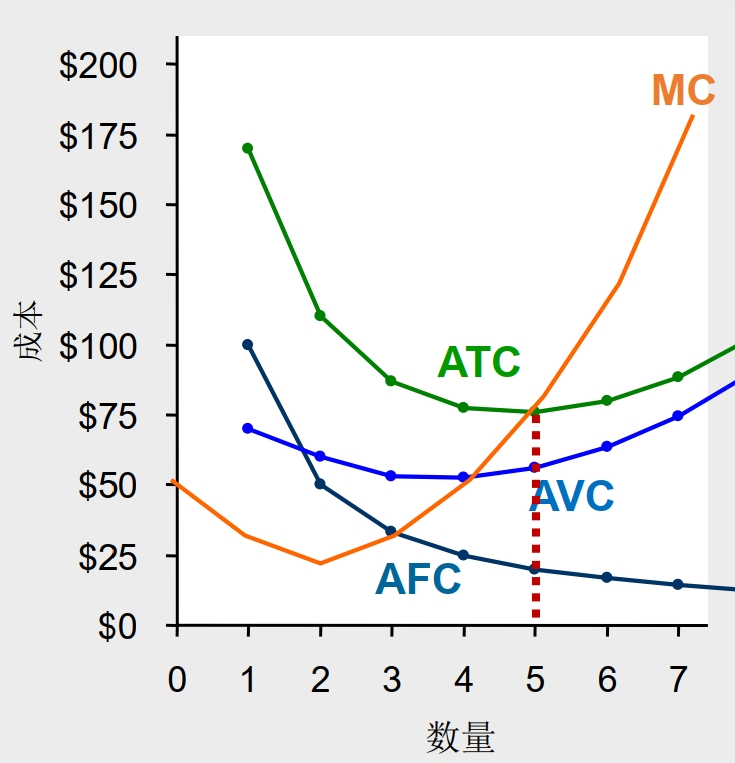
\includegraphics[width=0.4\textwidth]{各种成本曲线.png} 
  \caption{各种成本曲线} % 为图片添加标题
\end{figure}
当 MC < ATC, ATC 减少;当 MC > ATC, ATC 增加\\
\indent \textcolor{red}{MC曲线从ATC曲线的最低点处穿过}\\


企业的各种成本:\\
• 总成本、固定成本、可变成本\\
• 平均总成本、平均固定成本、平均可变成本、边际成本\\
• 边际成本从平均总成本和平均可变成本的最低点穿过\\
• 平均总成本最低的点对应的数量是企业的\textcolor{red}{有效规模(efficient scale)}\\
\[
ATC = \frac{TC + \Delta TC}{Q + \Delta Q};
AVC = \frac{VC + \Delta VC}{Q+ \Delta Q };
MC = \frac{\Delta TC}{\Delta Q } = \frac{\Delta VC}{\Delta Q };
\]
%7.3
\subsection{短期成本与长期成本}
%7.3.1
\subsubsection{短期与长期}

\begin{description}
  \item[短期 (SR: short run):] 一些投入的数量是固定的(比如,工厂,土地)。这些投入的成本是固定成本。
  \item[长期 (LR: long run):] 所有投入的数量都是可变的(比如,企业可以建造更多的工厂或者出售已建好的工厂)。在长期里,任何企业的产量都被调整为有效规模 — 即平均总成本最小的规模。
  \item[\textcolor{red}{长期平均总成本(LATC):}] 在任何低于QA的产量,企业在长期会选择规模 S;生产在QA与QB之间的产量,企业在长期会选择规模M;生产高于QB的产量,企业在长期会选择规模L 
\end{description}


\begin{figure}[H] 
  \centering % 使图片居中显示
  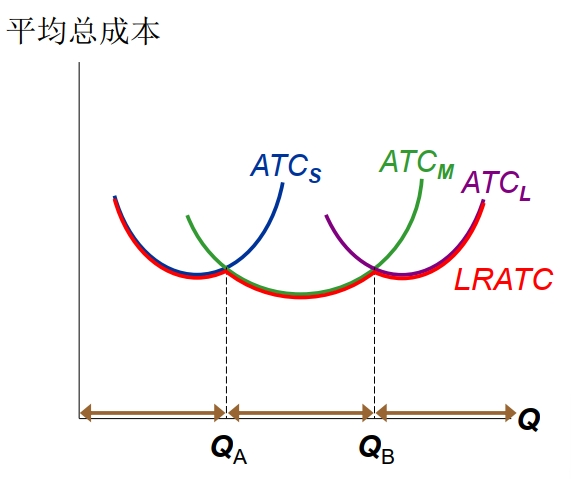
\includegraphics[width=0.4\textwidth]{长期平均总成本.png} 
  \caption{长期平均总成本曲线(LRATC)} % 为图片添加标题
\end{figure}

%7.3.2
\subsubsection{规模经济}

ATC沿LRATC变动的三个阶段:随Q增加,ATC下降、不变、增加。

\begin{itemize}
  \item \textcolor{red}{规模经济 (increasing return to scale)}:长期平均总成本随产量增加而减少。 产生原因是较高的产量水平允许工人实现专业化,例如,专业化可以使工人更精通某一项工作,如流水线上的工人。 通常在产量低时,规模经济更常见。

  \item \textcolor{red}{规模收益不变 (constant return to scale)}:长期平均总成本在产量变动时保持不变。

  \item \textcolor{red}{规模不经济 (decreasing return to scale)}:长期平均总成本随产量增加而增加。 规模不经济的产生是由于任何一个大型组织中固有的协调问题,例如,管理团队越庞大,管理协调困难;中央计划等。
\end{itemize}


\newpage
% Chapter 8
\section{竞争市场}

\subsection{什么是竞争市场}

\subsection{利润最大化}

\subsection{竞争企业的供给和需求曲线}

\newpage
% Chapter 9
\section{垄断和垄断竞争市场}

\subsection{什么是垄断}


\subsection{广告}



\end{document}